\subsection{Evaluation}
\label{emt:sec:eval}

\subsubsection{Methodology}
\label{emt:sec:eval:metho}

\noindent
We validate the correctness of the EMT-Linux implementation
	using Linux tests.
Since EMT supports all virtual memory features in Linux,
	EMT-Linux % does not change the system call interface, userspace tests 
	should pass any userspace tests. 
	%  with both x86-64 Radix and ECPT MMU drivers.

We also measure the interface overhead of EMT by running 
	the same set of performance benchmarks on
	EMT-Linux (\S\ref{emt:sec:impl}) and 
	vanilla Linux running upon the same hardware.

We then measure the performance of EMT-Linux on ECPT. 
We run EMT-Linux with the ECPT MMU driver on top of an emulated ECPT MMU 
	using our emulation framework (\S\ref{emt:sec:eval:emulator}).
We compare the performance of EMT-Linux with the Radix MMU driver
	running on an emulated x86-64 MMU.

% Evaluating ECPT is challenging because 
%	there is not yet a hardware MMU of the ECPT architecture.
% A common practice is full-system simulations (e.g., using Intel Simics~\cite{})
%	which is used by a few prior work~\cite{,}.
%We find it a common dilemma of new architecture research.
%Existing full-system simulations~\cite{} focus on hardware.
%To address this dilemma, we assemble an emulation framework (\S\ref{emt:sec:eval:emulator})
%	runs EMT-Linux on QEMU~\cite{qemu} 
%	with a software MMU where we implemented hardware logic of ECPT.
% The emulation framework allows hardware-software codesign and enables us to 
%	measure both software overhead of ECPT on Linux 
%	and full-system hardware simulation.
% Lastly, we verified the user space performance benefits 
%	of ECPT using hardware simulation as in~\cite{skarlatos2020ecpt}.
% This section focuses on discussing the software/OS perspective.

\para{Benchmarks.} %We use two benchmarks to measure system performance.
We use LEBench~\cite{bench:lebench} as a micro benchmark to measure
the performance of core OS operations such
	as page fault handling, context switching, and system calls. 
% \schai{\texttt{mmap}, \texttt{muunmap}, \texttt{fork}, \texttt{read}, and \texttt{write}, etc.} 
% \TODO{read/write?}
% Besides the
% microbenchmark that evaluates the page fault handling of file-backed pages, we
% add two microbenchmarks for anonymous pages: one for the base page and the other
% for the huge page

% \begin{table}
% 	\centering
% 	\footnotesize
% 	\setlength{\tabcolsep}{4pt}
% 	%	\vspace{-5pt}
% 	\caption{\bf Macrobenchmarks used in the evaluation.}
% 	\vspace{-5pt}
% 	\begin{tabular}{|l|l|}
% 	\hline
% 		\textbf{Name} & \textbf{Description}  \\
% 		\hline
% 		\hline 
% 		\multirow{2}{*}{Breadth-first Search (BFS)} & In-memory key-value store (working-set: 8.5 GB) \\
% 		& 512M 256B records, 30M operations, 100\% reads \\
% 		\hline 
% 		\multirow{2}{*}{Depth-first Search (DFS)} & In-memory key-value store (working-set: 8.5 GB) \\
% 		& 100M 1KB records, 10M operations, 100\% reads \\
% 		\hline 
% 		\multirow{2}{*}{Degree Centrality (DC)} & Random memory accesses (working-set: 8.5 GB) \\
% 		& 128 GB dataset, 1B operations, 100\% updates \\
% 		\hline 
% 		\multirow{2}{*}{Shortest Path (SSSP)} & Data structure evaluator (working-set: 8.5 GB) \\
% 		& 1.5B keys, 70M operations, 100\% lookups \\
% 		\hline 
% 		\multirow{2}{*}{Triangle Count (TC)} & Chip design optimizer (working-set: 8.5 GB) \\
% 		& 100M elements, 150K swaps/step, 2K start temp. \\
% 		\hline 
% 		\multirow{2}{*}{Page Rank (PR)} & Chip design optimizer (working-set: 8.5 GB) \\
% 		& 100M elements, 150K swaps/step, 2K start temp. \\
% 		\hline 
% 		\multirow{2}{*}{Sysbench} & Monte Carlo simulator (working-set: 64 GB) \\
% 		& 170K gridpoints per nuclide, 4M particle histories \\
% 		\hline
% 		\multirow{2}{*}{GUPS} & Graph analysis benchmark (working-set: 64 GB) \\
% 		& 27 scale, 32 edge factor, 4 iterations \\
% 	\hline
% 	\end{tabular}
% 	\label{emt:table:workloads}
% \end{table}

We use nine memory-intensive macro benchmarks
	that stress the TLB and need off-TLB translation.
We use the same set of macro benchmarks from the ECPT paper~\cite{skarlatos2020ecpt,jovan2022nestedecpt}
	except two where we failed to reproduce the working set.
%\schaic{This claim is a bit dangerous here; we remove two benchmarks (BC and Mumer) since we cannot reproduce their working set}.
The macro benchmarks include seven applications from the GraphBIG benchmark suite~\cite{bench:graphbig}: 
	Breadth First Search (BFS), 
	Depth First Search (DFS), 
	Degree Centrality (DC), 
	Single Source Shortest Path (SSSP), 
	Connected Components (CC), 
	Triangle Count (TC), and PageRank (PR); they use the LDBC-1000K dataset~\cite{bench:graphbig-LDBC}, 
	with working sets of about 8.5 GB. 
We also run the GUPS benchmark~\cite{bench:gups} which issues random memory updates,
	and a memory test from Sysbench~\cite{bench:sysbench}. Both GUPS and Sysbench
	have 64 GB working sets.

We also evaluate three memory-intensive applications:
	Redis, Memcached, and PostgreSQL.
Table~\ref{emt:table:workloads} shows the workloads.
All these applications are multithreaded programs.
% Several benchmarks are multithreaded, including fork, tr.create, etc 
%	in LEBench as well as Redis, Memcached, and Postgres.

% \TODO{ % BEGIN TODO
% \jyk{TODO: Move it to the proper subsection.}
% Besides, measuring end-to-end
% execution time of the benchmarks, we also use perf to record their page walk
% latency to further collaborate our findings. For each kernel tested, all
% execution time and page walk latency numbers are collected under two
% configurations: with and without Transparent Huge Page (THP) enabled.
% } % END TODO

\subsubsection{Functional Correctness}
\label{emt:ss:correctness}

\noindent
We show that EMT supports all memory management features of Linux
	by running Linux Test Project (LTP)~\cite{tool:ltp} against EMT-Linux.
\schai{We use the default kernel configuration for the generic kernel (5.15.0-125-generic) of Ubuntu 20.04.}
LTP includes 1,405 tests in total and 1,208 of them apply to the kernel configuration.
% Each test is a user-space program that interacts with the kernel via system calls.
EMT-Linux with Radix, ECPT\schai{, and FPT} MMU drivers both pass all 1,208 tests
	which covers 376 system calls.
% \schai{EMT-Linux is compiled with the standard Linux toolchain with gcc -O2 optimization.}
% \schaic{Also report how many syscalls we tested?}
We also cross-validated program outputs of the micro and macro benchmarks
	across EMT-Linux and vanilla Linux.
We use testing as a continuous effort throughout our development,
	rather than a one-time effort, which
	helped capture bugs in a timely manner.

% introduced by refactoring, e.g., code that 
%	incremented pointers to
%	iterate page table entries that were not changed to the EMT interface.
%	and thus pointing to wrong entries in ECPT.
% \TODO{@Alan, is there any interesting bugs to share?}

% vanilla: 1208 passed 179 skipped 18 failed
% We run the validated 1,208 test cases with \eradix and \eecpt to check the
% correctness of the EMT. 

% \mmudrivers of \eradix and \eecpt support huge pages with THP \jyk{TO CHECK: Has
% it already been cited before.} and does not support HugeTLB Page interface of
% Linux yet. We turn off the HugeTLB flag of system calls, \texttt{futex},
% \texttt{futex\_wake}, \texttt{memfd\_create}, \texttt{move\_pages},
% \texttt{pkey}, \texttt{sbrk}, and \texttt{shmget}. THP is enabled system-widely
% to support huge pages in our testbed. With this configuration, both \eradix and
% \eecpt pass all 1,208 test cases correctly.

% Original text
	
	% We start with the memory system calls, specifically the mmap call, that
	% cause a non-deterministic kernel panic. The kernel panics that occurred
	% were due to malformed page table entries being read by the kernel
	% triggering a kernel panic. Specifically sometimes when calling the
	% `vfs\_read` function we would get a bad PTE kernel panic. However, we
	% found that this error only occurred sometimes, furthermore, in the debug
	% output and initial stack trace nothing appeared incorrect. After further
	% analysis, in the function `pagemap\_pmd\_range`, we found a for loop
	% that iterated through the various page table entries but didn't use the
	% generalized EMT interface but instead used `++`. This would cause the
	% kernel to sequentially iterate across the ECPT page table. This is an
	% issue since ECPT does not organize the page table entries contiguously
	% which means sometimes it may be the case the kernel reads bad memory.
	% After applying a fix to use the generalized EMT interface we fixed the
	% mmap system call. Since there are a lot of locations that need to be
	% switched to the EMT interface it is easy to miss locations that need to
	% be changed when switching to the EMT interface. \TODO{Future kernel
	% programmers should be cautious and make sure they catch all the
	% locations that need to be switched to the EMT interface.}
	
	% We moved on to fixing the file system calls. We found that several
	% system calls like fsconfig, fsync, ftruncate, etc. were all failing the
	% LTP test cases. We found that there were several reasons for these
	% system calls failing. On closer inspection it was clear that our testing
	% environment was not setup properly causing an early error return since
	% the LTP test case was unable to open the `/sys` file. Upon mounting
	% sysfs we found that several of these errors disappeared. In fact we
	% found that many errors were specifically due to misconfiguring of the
	% special ECPT vm. We also found additional issues with fsconfig, this
	% failure was due to a missing kernel patch that resulted in an integer
	% overflow. After applying the patch we fixed this test case. 
	
	% Moving onto the network system calls, we found that most of the 57
	% failed system call are actually in this category. The majority of these
	% failed system call test cases pointed to the connect system call failing
	% resulting in a cascading error. The issue with the connect system call
	% is that it always returns `ENETUNREACH` meaning no interface to connect
	% to. Upon analyzing the networking system call we trace the problem to
	% `\_\_ip\_dev\_find` finding no networks devices for the specific IP
	% address. We then scan our network devices to find that while there are
	% network devices, however, none of them have been assigned an IP address.
	% After fixing the vm environment to assign 127.0.0.1 to lo we are able to
	% fix the connect system call along with all the other system calls except
	% accept. Accept also required us to set up multicast support in the
	% special QEMU ECPT vm.

\subsubsection{EMT Interface Overhead}
\label{emt:sec:eval:eval-EMT-radix-vs-vanilla}

\noindent
EMT introduces negligible overhead.
We run the benchmarks and application workloads on vanilla Linux and EMT-Linux running on the same hardware.
The hardware is a dual-socket Intel Xeon Gold 6346 server at 3.10GHz
	with 16 cores and 256GB DDR4-3200 DRAM.
We disable hyperthreading and fix core frequency to make the measurement stable.
The overhead of EMT is calculated 
	by normalizing the results of EMT-Linux to vanilla Linux.
We experimented with various kernel configurations (e.g., enabling THP); the 
	results are consistent.

Figure~\ref{emt:fig:eval:microbenchmark} shows the results of \schai{kernel micro benchmarks} LEBench~\cite{bench:lebench}.
% \schaix{EMT-Linux shows negligible overhead over vanilla Linux.}	
\schai{EMT-Linux exhibits an average normalized kernel-routine performance of 99.9\% 
	relative to vanilla Linux (with a standard deviation of 1.1\%) across the 41 LEBench microbenchmarks.}
% The largest overhead comes from ``2MB anonymous page fault'',
% 	where EMT slows the benchmark by 4.91\%;
\schai{The largest overhead comes from the ``epoll big'' benchmark,
	where EMT-Linux slows the benchmark by 4.2\%.
% It was caused by operations that unmap file backed pages one by one,
% 	where each of them setups the iterator to unmap a single page.
% It could be further optimized if we expose a customizable function to unmap a single page.
% \schaic{This is a bit confusing, since we are not unmapping file backed pages one by one.}
	}
	It was caused by not inlining certain functions %\jzx{(the iterator functions)} 
	due to %\jzx{dependencies}{
	coding style restriction, %~\cite{linux:code:icache}},
	which can be further optimized by restructuring the code or forcing inlining.
% \begin{figure}[t]
% 	\centering
% 	%\vspace{-12.5pt}
% 	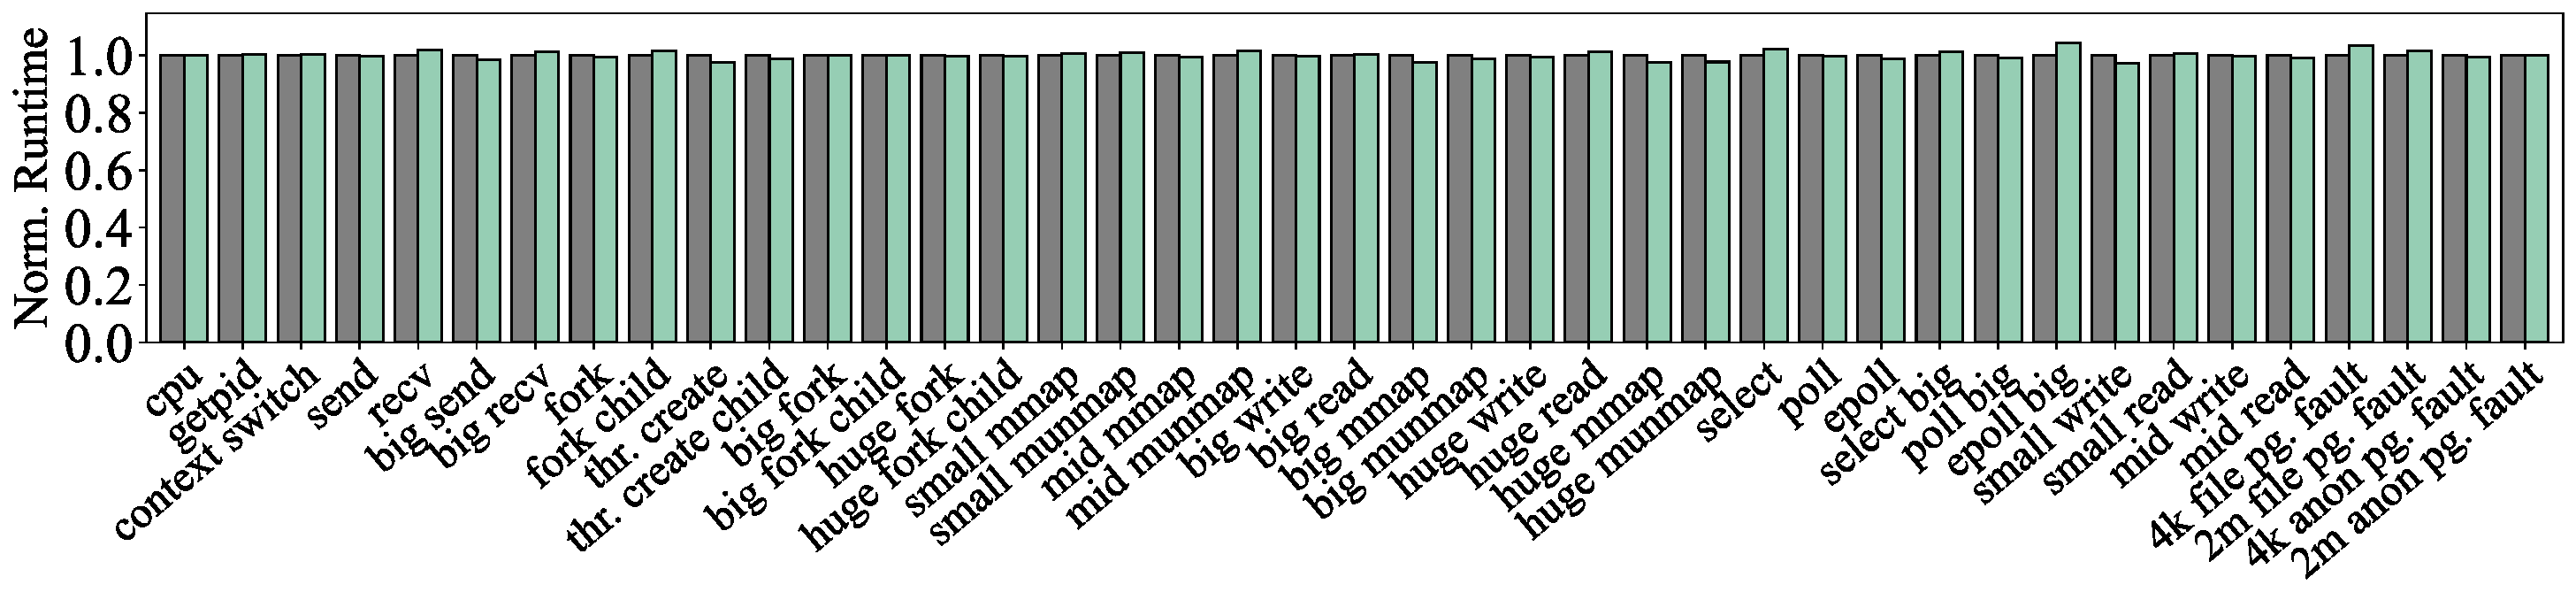
\includegraphics[width=0.7\textwidth]{data/radix_lebench.pdf}
% 	\caption{\bf Speedup of kernel micrombenchmarks execution in 4KB setup of \eradix over vanilla Linux. 
% 	\jyk{Replace Vanilla Linux bars
% 	with a line. It saves space.}}
% 	%\vspace{-15pt}
% 	\label{emt:figure:eval:eval-stack-lebench}
% \end{figure}
Figure~\ref{emt:fig:eval:macrobenchmark} shows that
	the overhead of EMT-Linux is less than 0.1\% on the macro benchmarks.
Figure~\ref{emt:fig:eval:eval-radix-real-app} shows the normalized throughput,
	average latency, and tail latency of three real-world applications (with workloads in Table~\ref{emt:table:workloads}) on 
	EMT-Linux, normalized to their performance on vanilla Linux.
The measured differences of the three metrics are within 
%  shows the performance of EMT-Linux on memory-intensive applications.
	0.1\%, 0.1\%, and 0.2\%, respectively.
\schai{The results of the real-world application show that 
	the EMT interface does not affect system responsiveness.}

\begin{table}
\centering
\footnotesize
\setlength{\tabcolsep}{4pt}
\begin{tabular}{lcccc}
\toprule
\textbf{Application} & \textbf{Working Set} & {\bf \# Records} & \textbf{Read:Write} & {\bf \# Requests} \\
\midrule
Redis      & 128 GB & 536 M & 50:50 & 60 M \\
Memcached  & 69 GB  & 56 M  & 80:20 &  10 M \\
PostgreSQL & 64 GB  & 21 M & 100:0 & 25 M \\
\bottomrule
\end{tabular}
\caption{\bf Application workloads used in the evaluation.}
\label{emt:table:workloads}
\end{table}

\begin{figure}[H]
	\centering
	% Legend subfigure
	\begin{subfigure}[b]{0.7\textwidth}
		\centering
		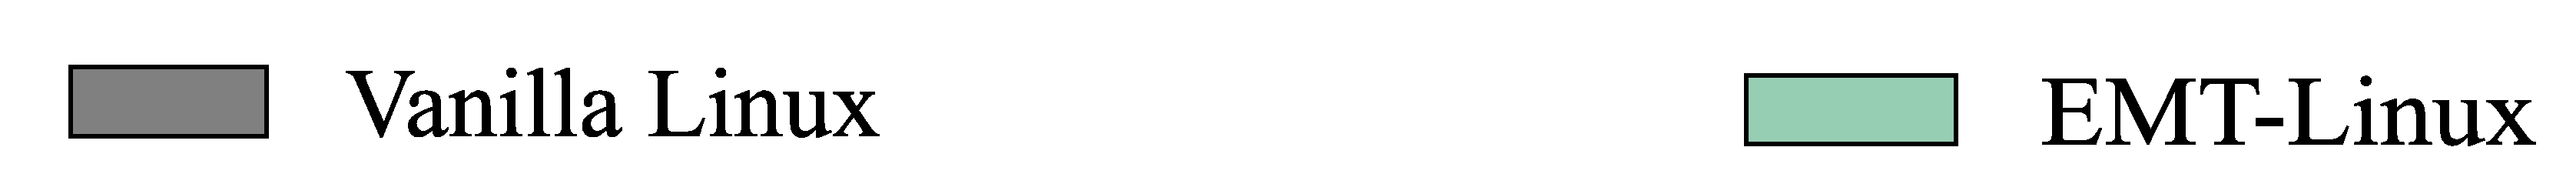
\includegraphics[width=\textwidth]{data/radix_real_app_legend.pdf}
		% 
\includegraphics[width=\textwidth]{data/radix_real_app_single_legend.pdf}
	\end{subfigure}


	% Subfigure 1
	\begin{subfigure}[b]{0.3\textwidth}
		\centering
		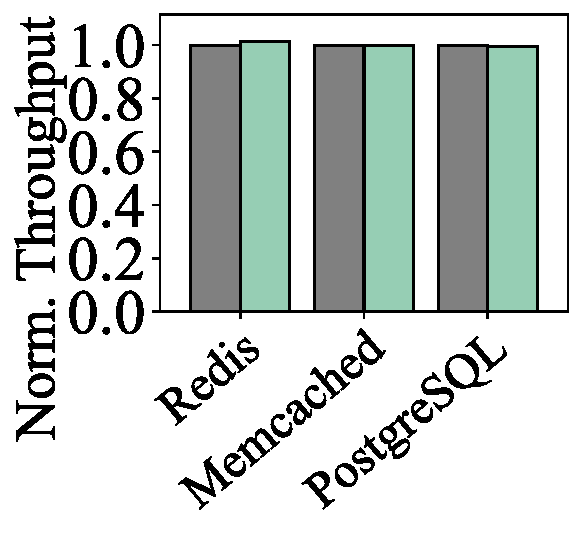
\includegraphics[width=\textwidth]{data/radix_real_app_throughput.pdf}
		% 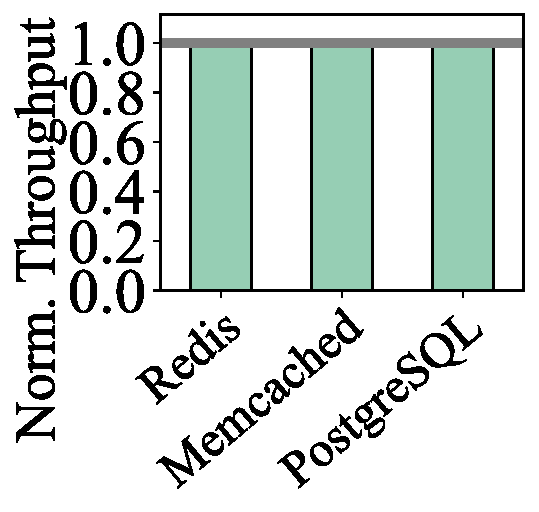
\includegraphics[width=\textwidth]{data/radix_real_app_throughput_single.pdf}
		\caption{Throughput}
		\label{emt:figure:eval:eval-radix-real-app-throughput}
	\end{subfigure}%
	% 
	\hspace{0.01\textwidth}%
	% Subfigure 2
	\begin{subfigure}[b]{0.3\textwidth}
		\centering
		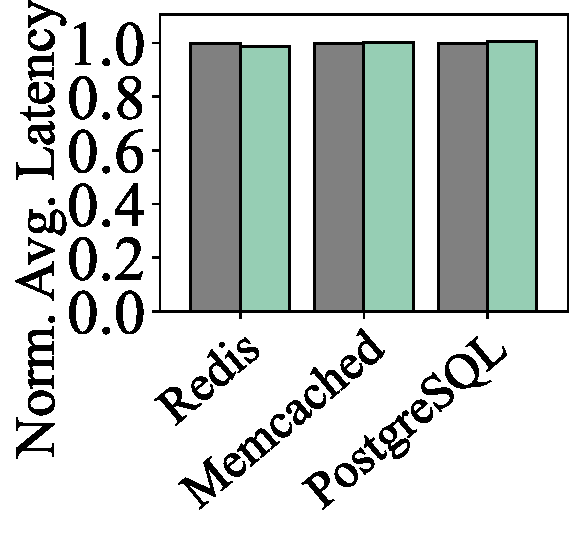
\includegraphics[width=\textwidth]{data/radix_real_app_avg_latency.pdf}
		% 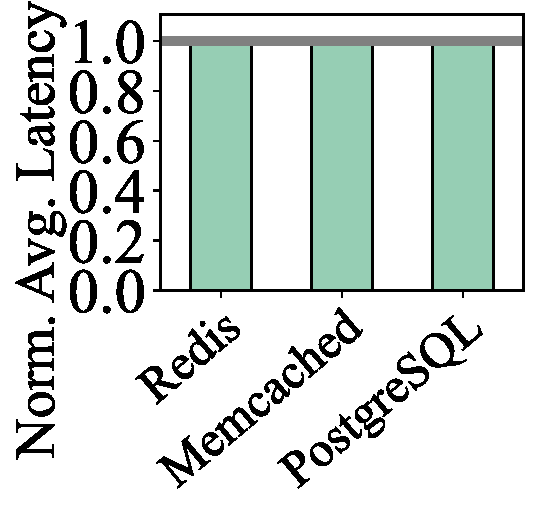
\includegraphics[width=\textwidth]{data/radix_real_app_avg_latency_single.pdf}
		\caption{Avg. Latency}
		\label{emt:figure:eval:eval-radix-real-app-avg-latency}
	\end{subfigure}%
	% 
	\hspace{0.01\textwidth}%
	% Subfigure 3
	\begin{subfigure}[b]{0.3\textwidth}
		\centering
		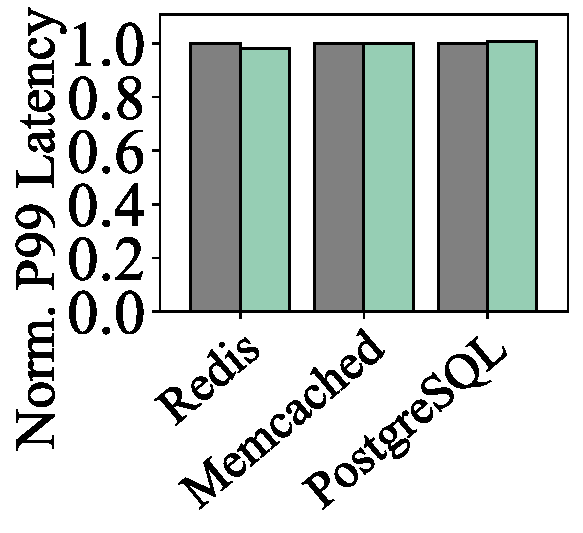
\includegraphics[width=\textwidth]{data/radix_real_app_p99_latency.pdf}
		% 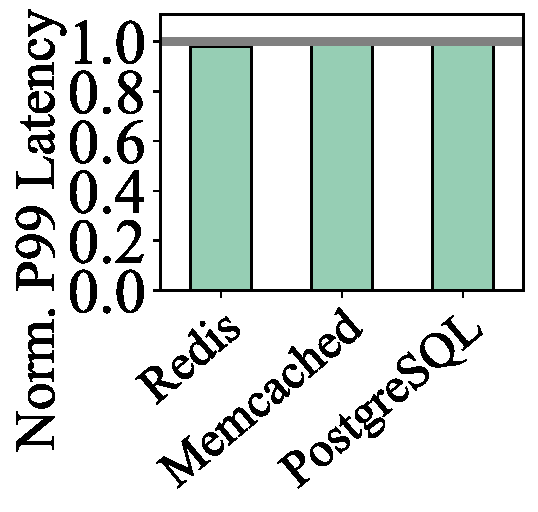
\includegraphics[width=\textwidth]{data/radix_real_app_p99_latency_single.pdf}
		\caption{P99 Latency}
		\label{emt:figure:eval:eval-radix-real-app-p99-latency}
	\end{subfigure}
	\caption{\bf Performance overhead of EMT-Linux over vanilla Linux
		on real-world applications}
	\label{emt:fig:eval:eval-radix-real-app}
\end{figure}

% On average, EMT adds a negligible overhead of 0.19\%.
% On average, the 
% on average, EMT takes 0.998571076652212 of the time

The negligible overhead is attributed to two kinds of endeavors.
First, we carefully engineered the EMT interface to preserve the 
	performance characteristics---we minimize increased stack size or deepened
	call stacks, and maintain cache efficiency.
% \schaix{The instruction cache hit rates on EMT-Linux are almost the 
% 	same as in vanilla Linux
% (more information can be found in Appendix~\ref{emt:appendix:perf})}.
% \schai{Instruction cache hit rates on EMT-Linux differ by at most 0.8\% from those on vanilla Linux (see Appendix \ref{emt:appendix:perf})}.
\schai{Instruction cache hit rates on EMT-Linux differ from those on vanilla Linux by at most 0.8\%.}
% (see Appendix \ref{emt:appendix:perf})}.
Second, EMT enables us to implement all the hardware-specific optimizations in the MMU drivers.

% We attribute it to the uses of compiler optimizations, 
%	cache efficiency (in cache hit rate), 
%	and principled uses of inline functions.
% In most cases, EMT does not deepen call stacks.
% On average, EMT-Linux is even faster than vanilla Linux---it takes 99.86\% of the time of vanilla Linux.
% \schaic{or we can say}
% \REVIEW{Overall, compared to vanilla Linux, EMT-Linux shows no obvious performance overhead 
% 	with an average performance difference of 0.14\%.}
% On average, EMT-Linux and vanilla Linux saves 0.14\% of execution time,
% 	which we consider as a negligible difference.

%	\schai{\texttt{addr\_range\_void} (Figure ~\ref{emt:code:thpgen})
%	since it is implemented in a different source file. 
%	It could be further optimized by putting the function into a header file to enable more inline opportunities.}
	% \TODO{inline a function due to XXX.}
% \schai{The overhead of EMT-Linux comes from the \texttt{addr\_range\_void} (Figure ~ref{code:thpgen})
%	function check in the page fault handler; 
% it is implemented in x86 MMU driver which makes cross translation unit function inlining not possible.}
% For huge pages, the average and the largest overhead are 0.25\% and 4.20\% respectively.
% For a few other benchmarks, \eradix outperforms vanilla Linux, e.g.,
%	EMT-Linux executes ``huge mmap'' 6.13\% faster 
%	and ``select'' 5.62\% faster.
% For the other micro benchmarks, the difference is within the standard deviation.
% We find these two have high standard deviation in the results.
% ``huge mmap'' has coefficients of variation (standard deviation over mean) 
%	13.61 and 4.42 for vanilla and genx86, respectively.
% ``select'' has 14.27 and 10.27 for vanilla and genx86, respectively.
% With such wide variation, we cannot conclude that EMT is faster than vanilla Linux.

% On average, EMT-Linux takes 99.96\% of the time of vanilla Linux.
% \schai{Furthermore, all of the benchmarks introduce overhead les than 0.28\%.
%	% The results suggests that running on 
%	The macrobenchmarks has more stable performance trend than the microbenchmarks,
%		since benchmarks spend majority of time running userspace instructions.}
% \TODO{@Siyuan will add a new figure and we will talk about the throughput and average/tail latency there.
% EMT-Linux's throughput and P99 latency are 1.4\% and 0.19\% 
% 	higher than those of vanilla Linux.}


% The reason why that EMT-Linux has a more stable performance trend in macrobenchmarks and memory intensive applications is that
%	the major kernel activities are in 4K anonymous page fault handler (as shown in Figure~\ref{emt:fig:eval:eval-kern-inst-breakdown}).
%	EMT-Linux's performance difference is only of 0.5\% according to measurements from microbenchmarks in Figure ~\ref{emt:fig:eval:microbenchmark}.


% EMT's negligible overhead is attributed to the implemenation of extensively using 
%	macro expansions over function calls to avoid runtime overhead.


% 7 times run & arithmetic average
% \schaic{The bars are the from seven times arithmetic avearge (geo mean doesn't make too much differen here though).}
% Overhead worst: 6.126% for 4KB, 5.129% for THP
% Average speedup: 0.189% for 4KB, 0.251% for THP
% Speedup best and worst: 
	% For 4KB case, the largest speedup is huge mmap (1.06126 speedup). 
	% The slowest is 2M anon pg. fault (0.9532 speedup). 
	% For THP case, fastest is 1.0612 speedup for thr create,
	% and slowest is 0.9580 for fork Child.


% Compared with Vanilla Linux, \branding does not add performance overhead to
% kernel operations (Figure ~\ref{emt:figure:eval:eval-stack-lebench}). The correct
% results and on-par performance of \eradix also confirms the \branding's
% comprenhensiveness and implementation's correctness to support Linux's various
% memory related syscalls and routines like page fault handler and context switch.
% \eradix's performance difference with vanilla on kernel micrombenchmarks is
% within 6.126\% under 4KB pages, and 5.129\% with THP enabled.
% 
% \schaic{We can choose report average performance speedup/slowdown or performance bounding like this.}
% On average, \eradix has performance difference of 0.189\% with Linux Vanilla
% 	when only 4KB pages are used.
% With THP turned on, the average performance difference is 0.251\%.
% \jyk{Are the the bars the average value of multiple-time runs?}
% \schaic{Yes, the bars are the from seven times arithmetic avearge (geo mean doesn't make too much differen here though).}
% \jyk{I see some cases that we achive better performance than the vanilla. What is the best percentage of them? And Why we get better numbers? Due to some optimizations or efficient path?}
% \schaic{For 4KB case, the largest speedup is huge mmap (1.06126 speedup). 
% 	The slowest is 2M anon pg. fault (0.9532 speedup). 
% 	For THP case, fastest is 1.0612 speedup for thr create,
% 	and slowest is 0.9580 for fork Child.
% 	The slow part makes sense since our interface adds a bit overhead in aspace checking,
% 	but I may need to check the fast part further.}



% The memory intensive applications shows similar but more stable performance trend as kernel micrombenchmarks.
% The stability comes from applications' longer running time
%	and the fact that they spend only part of time in kernel.
% \eradix's end-to-end performance difference with vanilla is within 0.276\% under 4KB pages 
%	and 0.177\%  with THP enabled.
% For page walk latency, \eradix's difference with vanilla is within 0.350\% with 4KB pages
%	and 1.402\% with THP enabled.

%\begin{figure}[h]
%	\centering
%	%\vspace{-12.5pt}
%	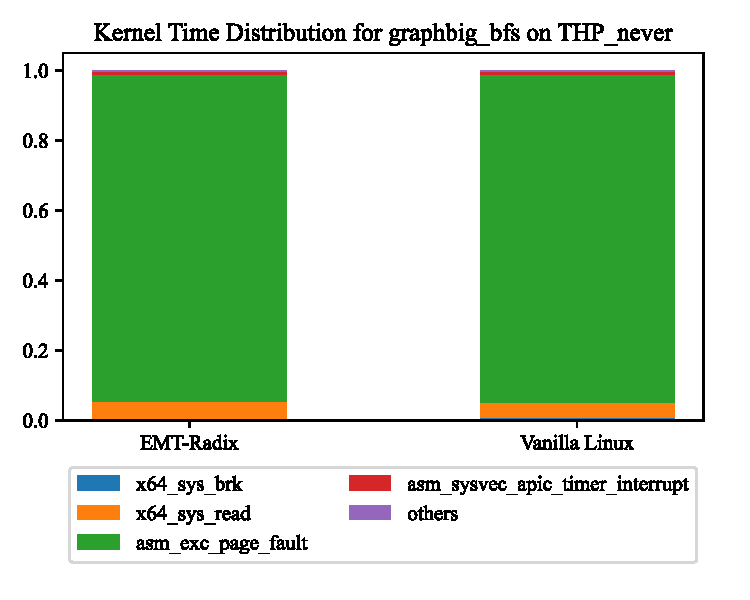
\includegraphics[width=0.49\textwidth]{data/THP_never_graphbig_bfs}
%	\caption{\bf Kernel Time Distribution of \eradix and Linux Vanilla for
%	graphbig\_bfs \jyk{@Siyuan, Please draw this figure with horizontal
%	bars. It will save space.}}
%	%\vspace{-15pt}
%	\label{emt:figure:eval:eval-bfs}
% \end{figure}

\begin{figure}[tbp]
	\centering
\begin{subfigure}[b]{0.7\textwidth}
	\centering
	
\includegraphics[width=\textwidth]{data/kern_inst_legend_cropped.pdf}
\end{subfigure}%
\vskip\baselineskip
\begin{subfigure}[b]{0.48\textwidth}
	\centering
	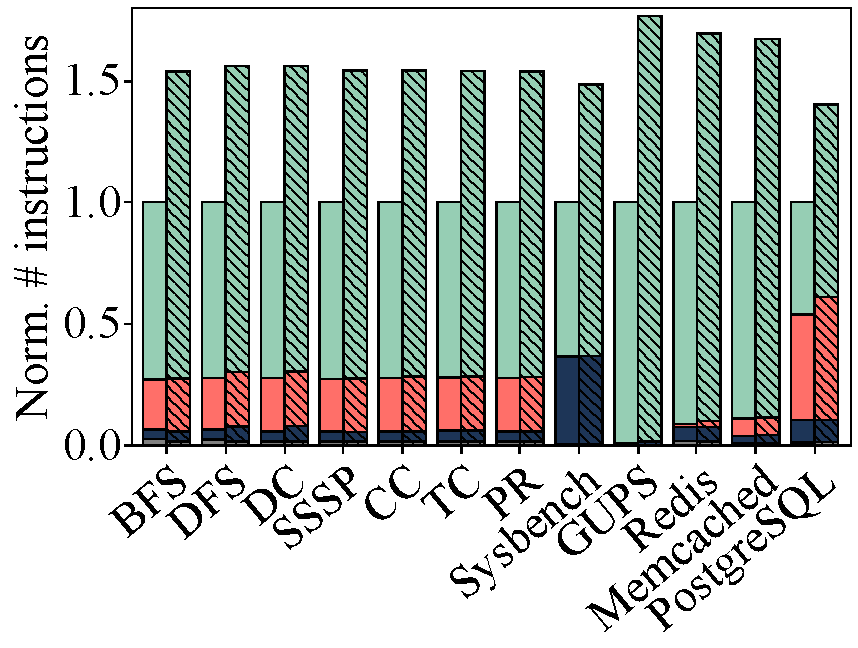
\includegraphics[width=\textwidth]{data/kern_inst_unified_never.pdf}
	\caption{4KB}
	\label{emt:figure:eval:eval-kern-inst-breakdown-4k}
\end{subfigure}%
\hspace{0.01\textwidth}
\begin{subfigure}[b]{0.48\textwidth}
	\centering
	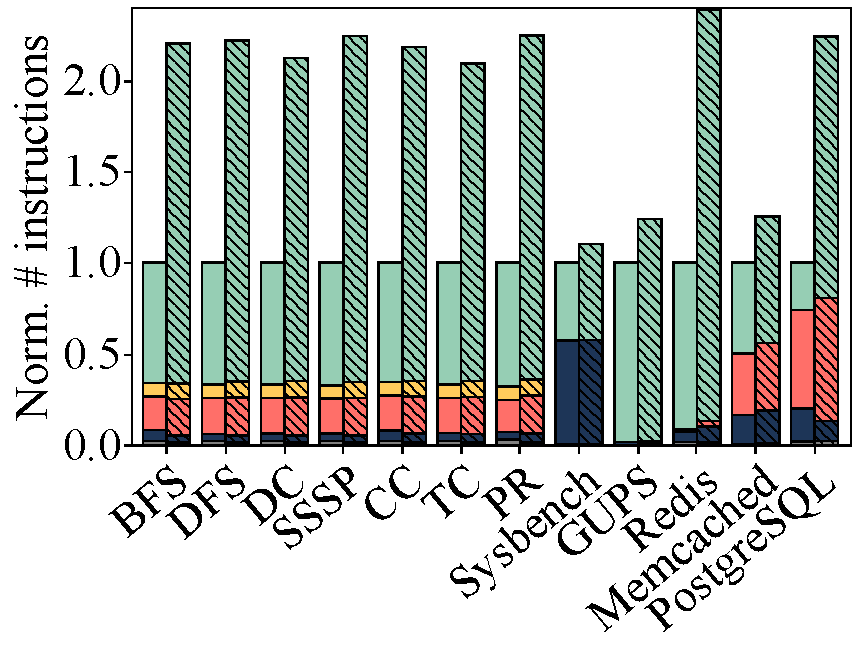
\includegraphics[width=\textwidth]{data/kern_inst_unified_always.pdf}
	\caption{THP}
%	\schaic{We redo sub figure c with a more complete optimization in iterator. 
%	The iterator used to do a lookup if current pte pointer is not valid (prev lookup not found entry in ECPT).
%	With this version, we avoid doing a lookup by just let the caller know that current pte pointer is not valid as well.
%	In the end, I think we only need to keep subfigure c.
	\label{emt:figure:eval:eval-kern-inst-breakdown-thp-harsh}
\end{subfigure}
\caption{\bf Distribution of kernel instructions of EMT-Linux with the Radix and ECPT MMU drivers.}
\label{emt:fig:eval:eval-kern-inst-breakdown}
\end{figure}

\subsubsection{OS Performance on ECPT}
\label{emt:ss:perf-ecpt}

\noindent
We show that EMT enables us to understand OS performance
	on new translation architectures using ECPT as an example.
We evaluate ECPT by running EMT-Linux with the ECPT MMU driver on our emulation framework
	and comparing its performance with the x86-64 radix MMU driver.
% Table~\ref{emt:table:configuration} shows the hardware configuration we simluated,
%	which models the hardware server we use.
We run macro benchmarks and application workloads
	and record all kernel and user instructions (with both 4KB pages and THP). 
% and memory traces of the applications.
% The macrobenchmarks composed of two stages: 
%	1) loading stage where application prepares data or memory buffer,
%	and 
%	2) running stage where the application performs the main computation or memory updates.
% To analyze the kernel behavior,
%	we capture the kernel instruction traces during benchmarks's loading stage 
%	which involves more kernel activity.
% For each benchmark, we caputred the kernel traces while 
%	running a fixed amount of user work in the loading stage (capped by 2B user instructoins).
% Different from most of the benchmarking tools which focus on performance running stage of benchmark,
	% we analyze the its loading stage since it involves more kernel activity.
% We evaluate EMT-Linux with x86-64 Radix MMU drivers and ECPT MMU drivers with only 4KB pages 
%	and with THP (Transparent Huge Pages).

% \begin{figure}[h]
% 	\centering
% 	\vspace{-10pt}
% 	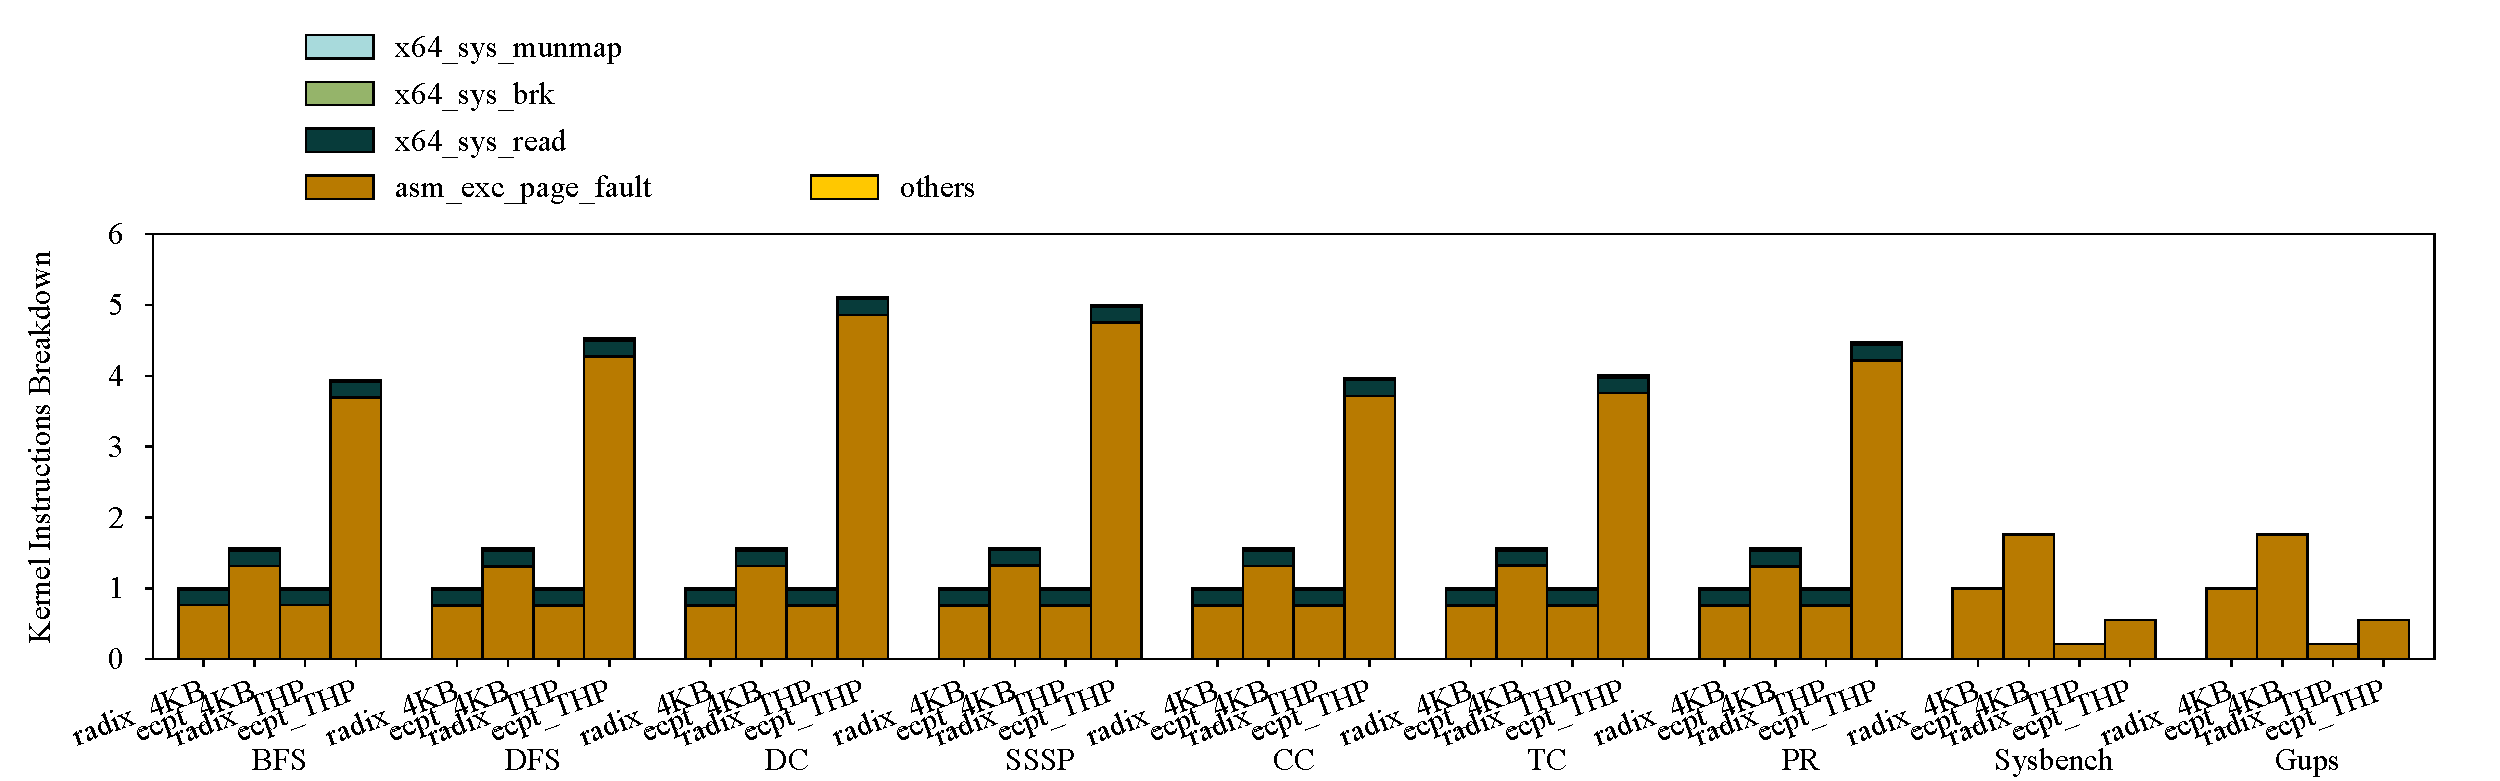
\includegraphics[width=0.49\textwidth]{data/kern-inst-grouped-stacked-bar.pdf}
% 	\caption{\bf Distribution of kernel instructions}
% 	%\vspace{-15pt}
% 	\label{emt:figure:eval:eval-kern-inst-breakdown}
% \end{figure}

% \begin{figure}
% 	\centering
% \begin{subfigure}[b]{0.5\textwidth}
% 	\centering
% 	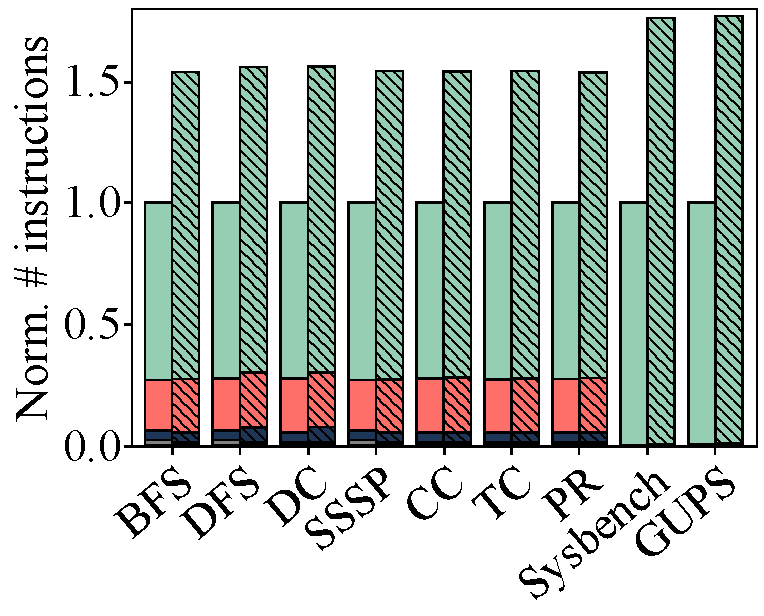
\includegraphics[width=0.5\textwidth]{data/kern_inst_never.pdf}
% 	% \vspace{-0.1cm}
% 	\caption{ 4KB}
% 	\label{emt:fig:eval:eval-kern-inst-breakdown-4KB}
% \end{subfigure}%
% 	% \newline % This starts a new line
% 	% Subfigure 2
% 	% \vspace{-2cm}
% 	% \vspace{0.1cm}
% 	% \vspace{pt}
% \begin{subfigure}[b]{0.5\textwidth}
% 	\centering
% 	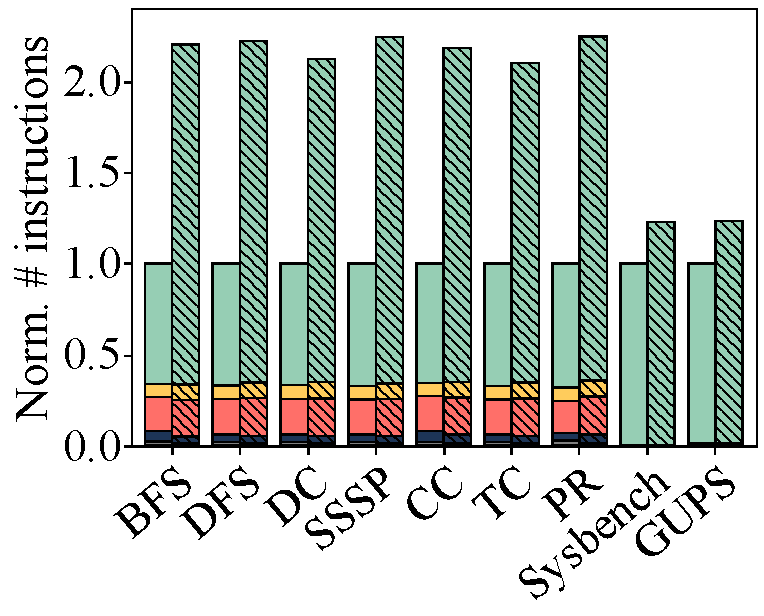
\includegraphics[width=0.5\textwidth]{data/kern_inst_always.pdf}
% 	% \vspace{-0.1cm}
% 	\caption{THP}
% 	\label{emt:fig:eval:eval-kern-inst-breakdown-thp}
% \end{subfigure}
% 	\caption{\bf Kernel instruction breadkown for 4KB and THP setup \eradix and \eecpt}
% \end{figure}

\para{Understanding OS Overhead of ECPT.}
\label{emt:ss:eval:eval-ecpt-os}
% The evaluation helps understand ECPT from the OS perspective.
Figure~\ref{emt:fig:eval:eval-kern-inst-breakdown} shows the distribution of kernel instructions;
	most of them are for page fault handling. % in our setup.
% Compared with Radix, ECPT spends 1.74x more instructions on page fault handling on average for 4KB pages,
% 	and 2.41x more with THP enabled. 
% data with unified appraoch: beginning of loading + running stage
Compared with Radix, ECPT spends 1.74x more instructions on page fault handling on average for 4KB pages,
	and 2.59x more with THP enabled. 
When THP is enabled, ECPT leads to relatively more work than Radix
	because Linux's THP implementation uses
	a few expensive operations to check
	if there exist valid entries in a given address range. % (\texttt{aspace\_partial\_built}).
% \schaic{This will be easier to understand if we provide code example, preferrablly in design/impl section}.
These checks are on the critical path of page fault handling when THP is enabled
	since the kernel needs to know if the 2MB range has any mappings % (huge page, directory of 4KB pages, or any 4KB pages)
	before it can decide if a 2MB huge page mapping should be built. % in PF handler.
% If any of the mappings exist, the kernel will resort other ways to handle the page fault (e.g. build 4KB pages or check properties)
%	rather than building a 2MB huge page mapping. \TODO{can't understand}
%	One major source of ECPT's kernel overhead 
%	is the \texttt{\small addr\_range\_void} function which takes 54.98\% of kernel instructions,
%		which iterates the surrounding address space of the faulting location to check if the page fault can be handled by allocating a THP.
For Radix, these checks are cheap (0.39\% of total kernel work)
	because a PMD entry has information on PTE tables. % (Figure~\ref{emt:fig:background:radix-native}).
If the entry is not valid or present, then neither 2MB nor 4KB mappings exist;
the huge-page bit tells if the entry points to a huge page or a directory of 4KB pages.
However, these checks are expensive in ECPT, as
	ECPT's entries are independent,
	the kernel may need to check all 512 4KB entries of pages in 
	the 2MB range, which requires many expensive lookup operations.
We discussed the potential solution % using special entries in PMD-ECPT 
	in \S\ref{emt:sec:reflection:sparse}.

% is to record the information in a special entry 
%	in the 2MB page table to avoid expensive checks.

\begin{comment}
\begin{table}
	\centering
	\scriptsize
	\caption{Percentage of Kernel instruction in total instructions}
	\begin{tabular}{|l|l|l|l|l|}
	\hline \textbf{Benchmark} & \textbf{x86 4KB} & \textbf{ECPT 4KB} & \textbf{x86 THP} & \textbf{ECPT THP}\\
	\hline 
	\hline
	GraphBIG average & 5.26\% & 7.98\% & 5.28\% & 11.28\%\\
	\hline
	Sysbench & 85.69\% & 91.38\% & 55.69\% & 60.72\% \\	
	\hline 
	Gups & 51.21\% & 57.69\%  & 18.03\% & 21.73\% \\
	\hline 
	\end{tabular}
	\caption*{\schaic{Should we include all graphbig benchmarks? the numbers are kind of similar, so I summarized as one row}}
	\label{emt:table:Kernel-inst-percentage}
\end{table}

\schaic{Actually, isn't radix a a better counterpart for ECPT? since x86 is typically referred as the entire x86 architecture.
and ECPT only changes its translation architecture part.
}

% Table ~\ref*{table:Kernel-inst-percentage} shows the percentage of kernel instructions in total instructions for the benchmarks.
% For graphbig benchmarks, the kernel instructions only account for a small part.
%	They try to read data from files during loading stage, so besides loading data into memory,
%		they also have to parse and format the data which involves more user instructions.
% In contrast, GUPS and Sysbench have significantly more kernel instructions since 
%	they faults in all the pages in memory during the loading stage.
% Figure~\ref{emt:figure:eval:eval-kern-inst-breakdown-4k} and Figure~\ref{emt:figure:eval:eval-kern-inst-breakdown-thp} 
%	show all of their kernel instructions are in page fault handling.

With THP enabled, Sysbench and GUPS spent less time in page fault handling
	since they can build huge pages in page fault handler,
	so given the same amount of memory size, less page faults are needed.
Yet, with THP enabled, GraphBIG benchmarks did not do less work
	because the benchmarks growing memory size dynamically as they loading more and more data from file.
In that situation, its vma size is always not enough for huge pages.
A potential optimization for the benchmark is to mmap huge chunks of memory at the beginning,
	so more huge pages can be utilized.
% }

	\jz{
		% which contributes \jztodo{100}\% of the total number of instructions executed on average for the workloads evaluated.
As shown, the heaviest kernel work is page fault handling,
	for 4KB setup it contributes 81.12\% and 87.69\% of the kernel instructions on average for x86 and ECPT respectively.
With THP enabled, it's 81.00\% and 91.59\% for x86 and ECPT respectively.
Also, compared to system calls such as \texttt{read}, \texttt{brk}, and \texttt{munmap},
	the page fault handler, which directly operates on page table,
	is more affected by the difference in translation architecture.
	}
\end{comment}

% Compared to x86, ECPT slows down the page fault handling by an average of \jztodo{100}\%,
% 	while system calls are largely not affected.}
% \TODO{How many are kernel instructions vs userspace instructions?
% What are the observations from Figure~\ref{emt:figure:eval:eval-kern-inst-breakdown}
% 	and what are the conclusions?
% Also, please improve Figure 13 as we discussed yesterday.} 

% \schaic{The plot ~\ref{emt:figure:eval:eval-kern-inst-breakdown} above needs to be modified in format, recapture loading phase data, as well as add gups and sysbench data}.
% \schaic{In loading phase, the timer effect will not be significant, so I feel acceptable to include timer. 
% However, in later phase, we exclude timer, I will remove it for now.}

% \TODO{can we parallelize this?}\JZc{Not likely, software-level parallelization requires IPI in this case, which could be more expensive}

% \JZc{Talk about given the result, for programs with frequent page faults, ECPT may not be an ideal design}
\begin{figure}[H]
	\centering
%\begin{subfigure}[b]{0.5\textwidth}
%	\centering
%	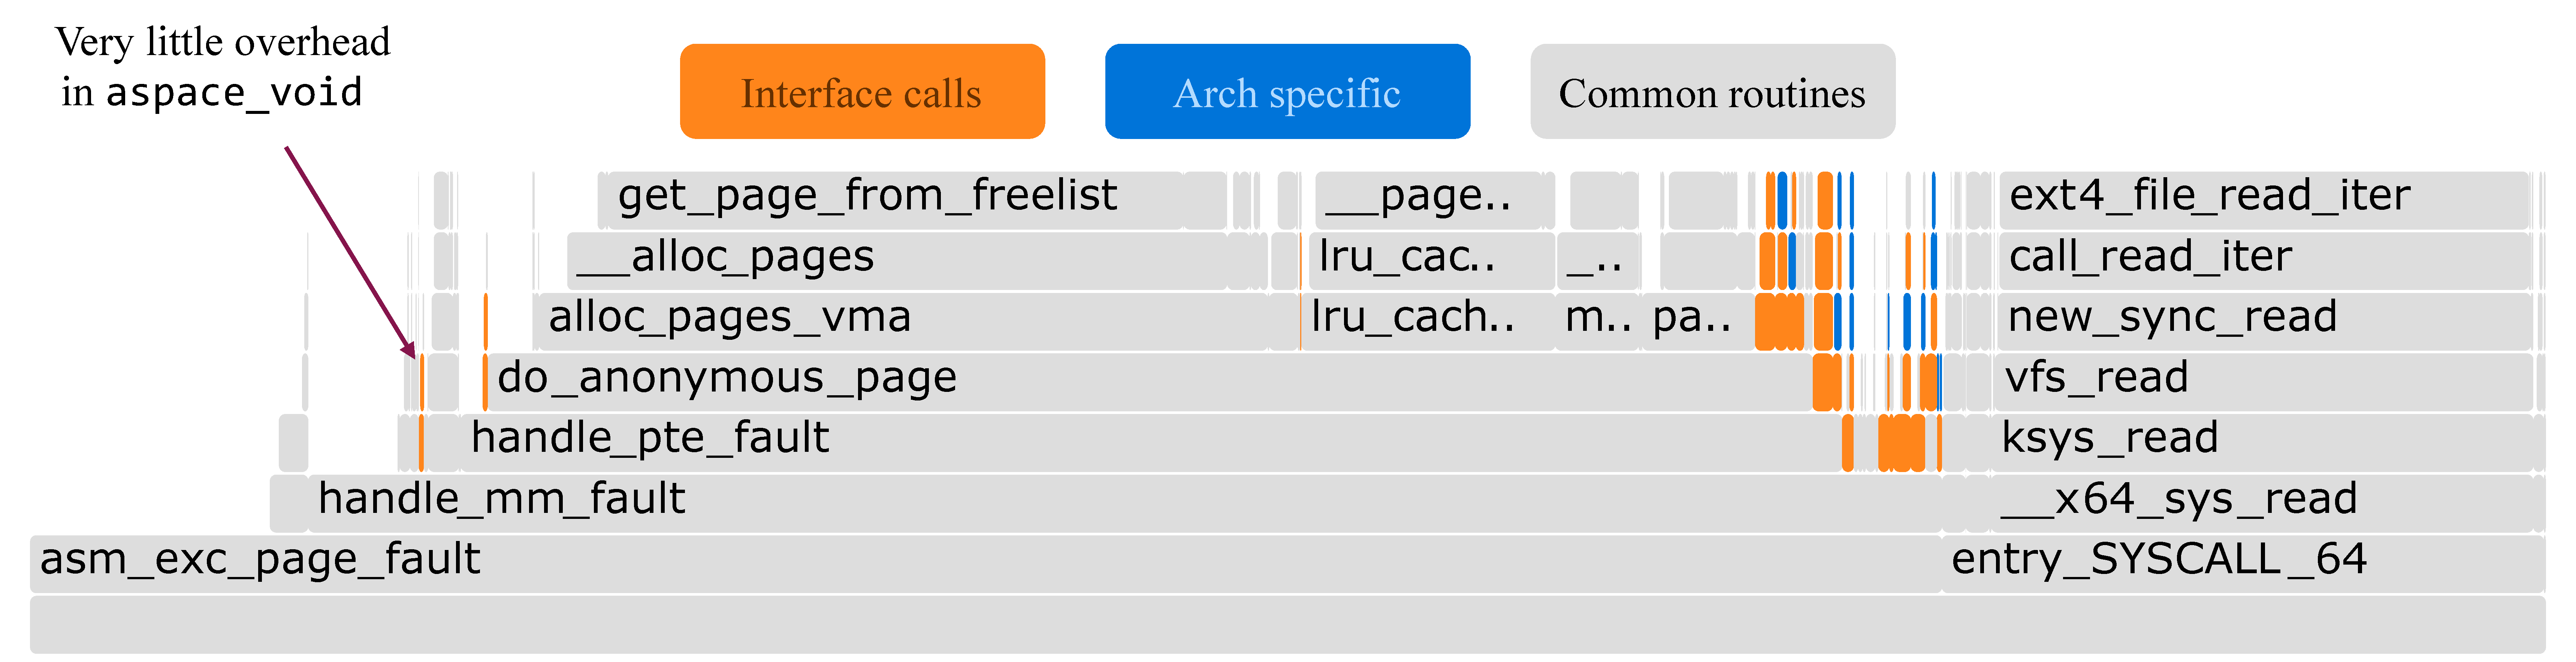
\includegraphics[width=\textwidth]{data/radix_always_graphbig_bfs_kern_inst.pdf}
%	% \vspace{-0.1cm}
%	\caption{x86-64 MMU driver}
%	\label{emt:fig:eval:eval-radix-always-vs-ecpt-always-flame-a}
\begin{subfigure}[b]{0.7\textwidth}
	\centering
	
\includegraphics[width=\textwidth]{data/flame_legend.pdf}
\end{subfigure}
\vskip\baselineskip
	\begin{subfigure}[b]{0.8\textwidth}
		\centering
		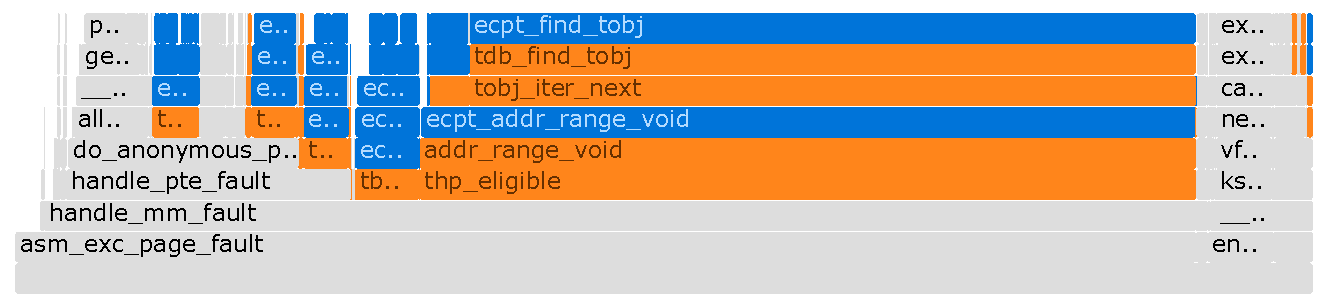
\includegraphics[width=\textwidth]{data/ecpt_always_graphbig_bfs_no_iter_kern_inst.pdf.corrected.pdf}
		% \vspace{-0.1cm}
		\caption{ECPT MMU driver with no iterator optimization}
		\label{emt:fig:eval::eval-radix-always-vs-ecpt-always-flame-a}
	\end{subfigure}

%	\end{subfigure}%
	% \begin{subfigure}[b]{0.5\textwidth}
	% \centering
	% 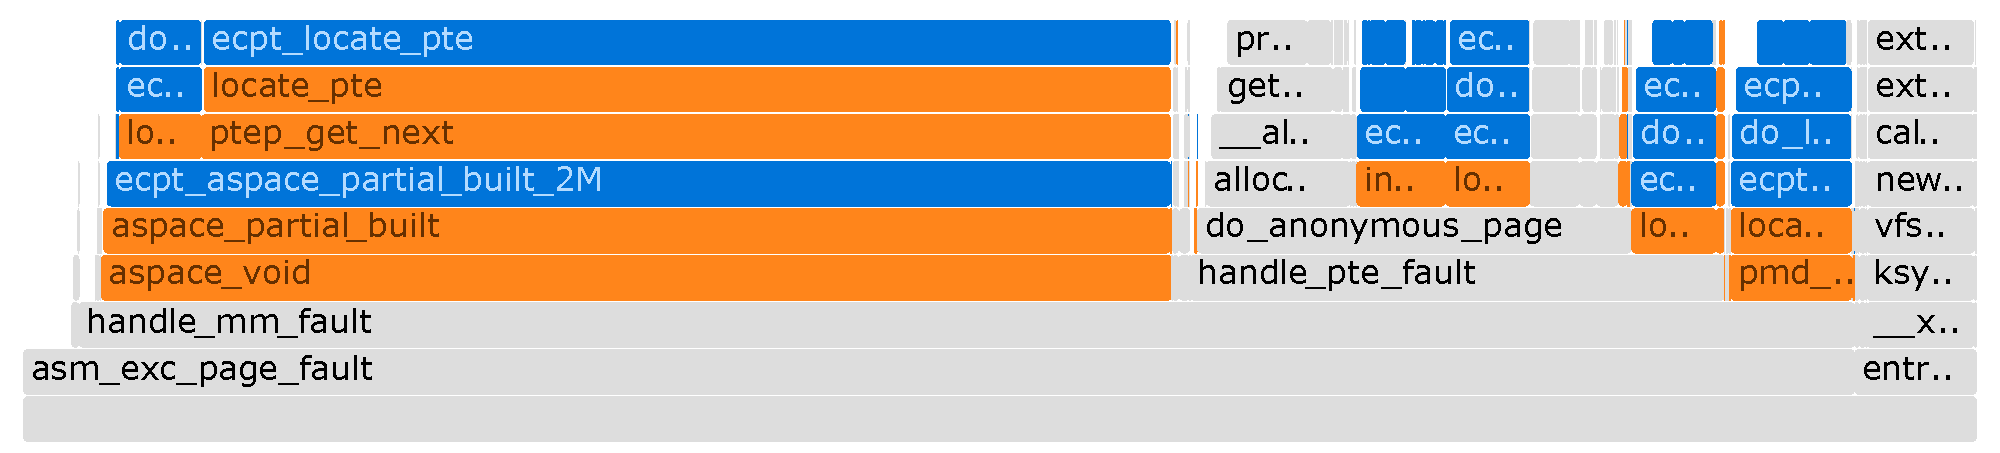
\includegraphics[width=\textwidth]{data/ecpt_always_graphbig_bfs_default_kern_inst.pdf}
	% % \vspace{-0.1cm}
	% \caption{ECPT MMU driver with incomplete iterator optimization }
	% \label{emt:fig:eval:eval-radix-always-vs-ecpt-always-flame-b}
	% \end{subfigure}
	\begin{subfigure}[b]{0.8\textwidth}
	\centering
	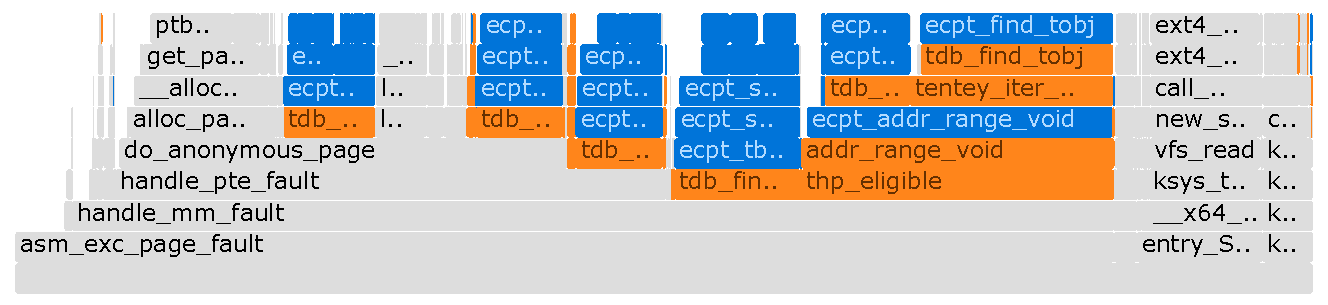
\includegraphics[width=\textwidth]{data/ecpt_always_graphbig_bfs_with_iter_kern_inst.pdf.corrected.pdf}
	% 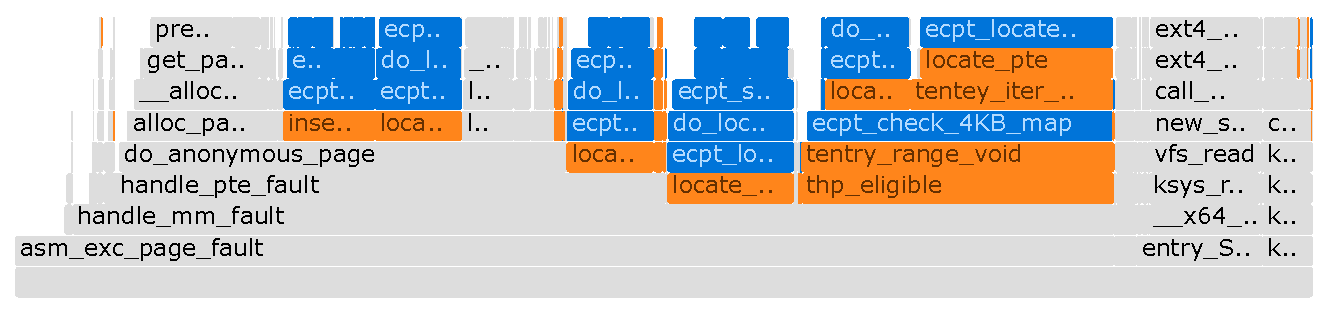
\includegraphics[width=\textwidth]{data/ecpt_always_graphbig_bfs_with_iter_kern_inst_cropped.pdf}
	\caption{ECPT MMU driver with iterator optimization
	% \schaic{The effect of subfigure c comes with more optimization from iterator.
	% 	The iterator used to do a lookup if current pte pointer is not valid (prev lookup not found entry in ECPT).
	% 	With this version, we avoid doing a lookup by just let the caller know that current pte pointer is not valid as well.
	% 	In the end, I think we only need to keep subfigure c.
	% }
	}
	\label{emt:fig:eval:eval-radix-always-vs-ecpt-always-flame-b}
	\end{subfigure}
	\caption{\bf Flame graph of EMT-Linux kernel instructions when running
	% \jyk{The scales(total number of instructions) of two graphs are different. Do we need to mention the number of instructions?}
	GraphBig BFS (THP enabled).}
	% \schaic{\texttt{aspace\_void} needs to be consistent}}
	\label{emt:fig:eval:eval-ecpt-flame-thp}
\end{figure}


\para{Effectiveness of Optimizations.}
% Before applying
% ECPT total 558,277,280
% ECPT PF 508,182,147
% aspace 285,024,081
% After applying sctricter iterator optimization.
% ECPT total 284,787,042
% ECPT PF 241,226,742
% addr range componnet 57,406,634
EMT exposes optimization opportunities for MMU drivers using customizable functions.
Figure~\ref{emt:fig:eval:eval-ecpt-flame-thp} uses flame graphs 
	to show the effectiveness of iterator optimization running 
	GraphBIG BFS with THP. % (we discuss another customizable function optimization in Appendix~\ref{emt:sec:app:another}).
With the iterator optimization (\S\ref{emt:ss:ecpt-mmu-driver}), 
	ECPT can save 
	% 47.27\%
	49.0\% 
	of total kernel work,
	and 
	% 49.97\% 
	52.5\%
	of the page fault handling work.
% Such saving comes from \texttt{addr\_range\_void} 
%	which iterate through the address range to check if the address range has any valid mappings.
% With iterator optimization, ECPT can save 79.86\% of its work in \texttt{addr\_range\_void}.
The optimization drastically saves the work of hashing and lookups of the architecture-neutral default implementation,
	by incrementing the pointer to an entry directly, as long as the entry is within an entry cluster (Figure~\ref{emt:fig:ecpt-impl:ecpt-cluster}).
% But, the optimized iterator is still significantly more expensive 
%	than that of Radix MMU driver.
% \TODO{talk about PWC -- see metareview}
Note that such kernel work as software overhead
	cannot benefit from hardware caches such as TLBs or PWCs.

% Furthermore, the breakdown also double confirms \branding's low overhead. 
% The overall instructions spent in \eradix's interface is 4.94\% of its kernel work,
%	while pure page table operations take 3.55\% of its kernel work.
% For \eecpt, the interface takes 38.42\% of its kernel work,
%	while pure page table operations take 38.25\% of its kernel work.	
% The little difference between \branding's interface work and pure page table operation work
%	not only corroborates our baremetal result in section \ref*{sec:eval:eval-EMT-radix-vs-vanilla},
%	but also shows that \branding's interface is lightweight even if the page table design is complicated.

% interface wrapped with radix 

% Radix total 112,504,629
% Radix PF 85,501,891

% ECPT total 442,685,858
% ECPT PF 415,046,832

% After applying sctricter iterator optimization.
% ECPT total 257,814,144
% ECPT PF 230,345,037
% addr range componnet

% \schai{With THP, EMT-Linux with ECPT does 2.29x more work overall and 
%	2.69x more work for page fault handling than with x86-64.
% In addition to ECPT's lookup and insert operations which contributes ECPT's more work in 4KB setup,
%	the other major source of overhead comes from 
%	\texttt{\small addr\_range\_void} function which takes 22.27\% of kernel instructions.	
% }

% The performance difference between \eradix and \eecpt is way more significant with THP enabled
%	than with 4KB pages.
% Part of the difference comes from overhead of ECPT's lookup and insert operations as the \eecpt with 4KB pages,	
% \TODO{@Siyuan: explain what the function does and why it's much more expensive in ECPT with THP.}
% \schaic{@Siyuan will make this more undstandable. but this is why it is more expensive in ECPT}

% The \texttt{\small addr\_range\_void} function needs to check multiple properties of a given adress range:
%	(1) if the range is mapped as a huge page,
%	(2) if the range is mapped as a directory of entries,
%	and (3) 

%	it runs a lookup for every next address.
% While the ECPT's optimized version can avoid the lookup 
%	if it can tell the next address is in the same cluster.
% It reduces the number of ECPT lookups
%	by exploiting PTE clustering and compaction design (Figure~\ref{emt:fig:ecpt-impl:ecpt-cluster}).
% Our retrofit of ECPT structure also makes this optimization possible
%	by making each PTE byte-addressable.
% Given that lookup is an expensive operation for ECPT,
%	iterator optimization can bring a great performance improvement.
% Such saving comes iterator optimization which reduces the number of ECPT lookups
% 	by exploiting the spatial contiguity of translation entries.
% Our iterator optimization enables MMU driver to take 

% \begingroup
% \setlength{\intextsep}{0pt}%
% \setlength{\columnsep}{4pt}%

% \begin{wrapfigure}{r}{0.2\textwidth}
% 	\centering
% 	\vspace{-25pt}
% 	% \hspace{-20pt}
% 	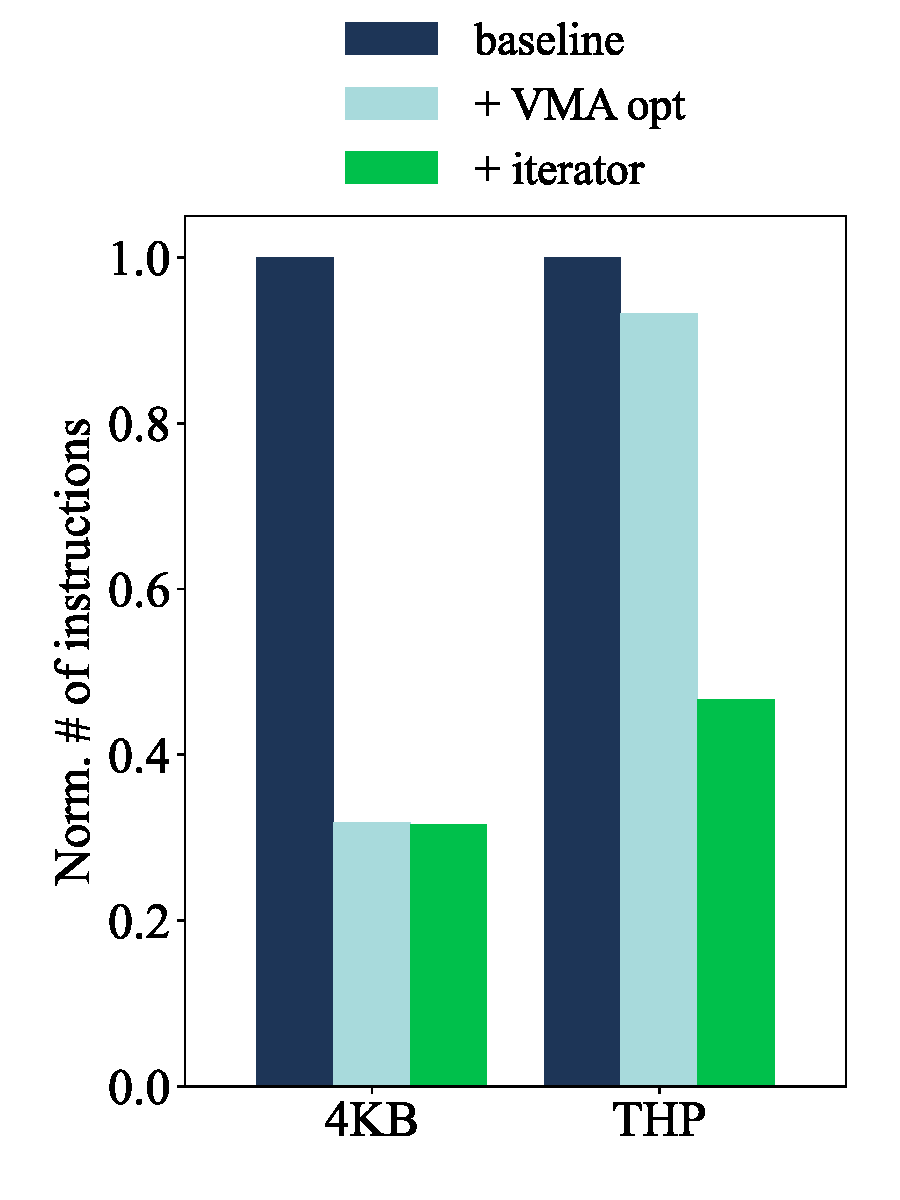
\includegraphics[width=0.2\textwidth]{data/opt_group_effect.pdf}
% 	\vspace{-15pt}
% 	\caption{\bf Effects of optimizations of page fault handling 
% 		with GraphBIG BFS.} 
% %	\schaic{The effect of subfigure is not so well, there're just too little nubmer of bars}}
% 	\label{emt:figure:eval:opt-group-effect}
% 	\vspace{-15pt}
% \end{wrapfigure}

\begin{comment}
\TODO{I don't see what Figure 14 shows, besides telling me that there is literally only
	one optimizations for the enture huge page group.}
% Under 4KB setup, the iterator, huge page and the combined optimizations 
%	reduce the number of instructions to 45.11\%, 31.87\% and 31.61\% of the baseline.
% With THP enabled, the iterator, huge page and the combined optimizations 
%	reduce the number of instructions to 48.34\%, 93.29\% and 46.67\% of the baseline.
We can see that the huge page optimization is the most effective one under 4KB setup,
	while the iterator optimization is the most effective one under THP setup.
The reason goes in how the page fault handler handles page faults under different setups.
% optimization reduces the number of instructions executed to  45.10\% of the baseline.
% The introduction of the hugepage optimization under this scenario 
% 	can further reduce the execution count to 31.61\% of the baseline. 
	% (Figure \ref{emt:figure:eval:opt-group-effect}a).
% With THP, the EMT-exposed optimizations reduce the kernel overhead by \jztodo{100}\% and then \jztodo{100}\%, respectively (Figure \ref{emt:figure:eval:opt-group-effect}b).

% code:iterx86
The page fault handler checks on \texttt{thp\_eligible}
	shown in Code snippet \ref{emt:code:thpgen} before it proceeds to build a huge page.
If \texttt{thp\_eligible} fails, the page fault handler
	will try to fix the page fault as 4KB fault or permissin fault.
It involves two checks:
	1) \texttt{\_\_transparent\_hugepage\_enabled} checks VMA's THP properties
	2) \texttt{addr\_range\_void} which checks if address range has any valid mappings.
For ECPT, 1) is much cheaper than 2) since 2) involves iterating through the address range
	as we mentioned in Section \ref{emt:ss:perf-ecpt}.

\begin{wrapfigure}{hr}{0.2\textwidth}
	\centering
	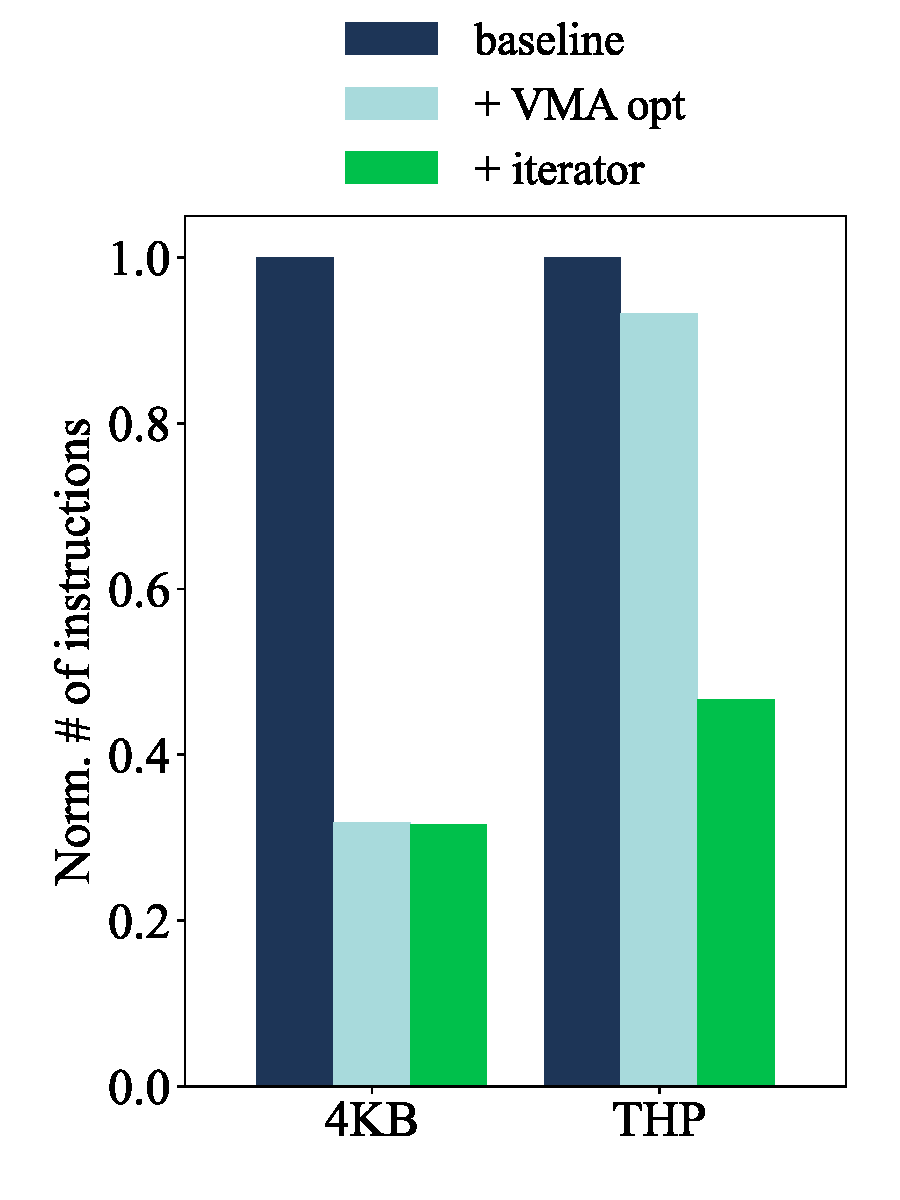
\includegraphics[width=0.2\textwidth]{data/opt_group_effect.pdf}
%	\vspace{-25pt}
	\caption{Effects of optimizations on BFS's PF handler.} 
%	\schaic{The effect of subfigure is not so well, there're just too little nubmer of bars}}
	\label{emt:figure:eval:opt-group-effect}
\end{wrapfigure}
Under 4KB setup, the check 1) will always be false because the VMA is not backed by huge pages. 
With huge page optimization, the page fault handler will skip the expensive address range iteration (check 2),
	and that explains the effectiveness of the huge page optimization under 4KB setup.
In contrast, under THP setup, the check 1) will be true for most VMAs,
	so the page fault handler cannot skip the expensive address range iteration
	even if we applied the huge page optimization.
In such case, the iterator optimization becomes ECPT's performance saver.
It utilizes the PTE clustering design of ECPT,
	effectively reduces the number of ECPT lookups 
	if it can tell the next address is in the same cluster.
\end{comment}

% With 4KB pages, huge page opt
% The overhead reduction mainly originated from the huge page handling part of the page fault handler,
% 	where expensive iterating and checking can be optimized.
% To be specific, with customizable functions,
% 	the ECPT MMU driver can perform faster iterations
% 		by exploiting the spatial contiguity of translation entries within a PTE cluster (\S\ref{emt:sss:ecpt-cluster})
% 			and thus avoiding redundant hash computations.
% Further, as shown in Figure \ref{emt:code:thpgen}, the ECPT MMU driver can optimize the eligibility checker
% 	to shortcut expensive range operation when THP is not possible,
% 		bringing in additional benefits.
% Hence, with 4KB pages only, as huge page operations are more frequently shortcutted,
% 	the effect of the hugepage optimization is more pronounced.

\begin{comment}
\paragraph{Page walk latency}
\label{emt:ss:eval:eval-pw}

% \begin{comment}
\begin{table}
	\centering
	\scriptsize
	\caption{Hardware configuration of the experiment machine.}
	\begin{tabular}{|l|l|}
	\hline \textbf{Parameter} & \textbf{Configuration} \\
	\hline
	\hline 
	Cores/Threads & 16 cores; 16 threads \\
	L1I TLB       & 64 entries, 8-way associative \\
	L1D TLB 	  & 64 entries, 4-way associative \\
	L2 STLB 	  & 1024 entries, 8-way associative \\
	L1I Cache 	 & 32 KB per core, 8-way associative, 2 cycles roundtrip (RT) \\
	L1D Cache 	 & 32 KB per core, 8-way associative, 2 cycles RT \\
	L2 Cache 	 & 512 KB per core, 20-way associative, 16 cycles RT \\
	Last-Level Cache & 16 MB, 16-way associative, 56 cycles RT \\
	Main Memory & 200 cycles RT \\
	Page Walk Cache & 3 levels, 2-4-32 entries per level, 1 cycles RT \\
	\hline
	\end{tabular}
	\label{emt:table:configuration}
\end{table}
% \end{comment}
Our framework also enables us to measure MMU's page table walk latency
	by replaying memory-traces in the DynamoRIO simulator.
% ECPT is modified with two optimizations to help improve performance, early return and parallel page walk cache access. 
Figure~\ref{emt:fig:eval:eval:pw-4KB} and ~\ref{emt:fig:eval:eval:pw-thp} shows the speedup of page table walk latency
	of a ECPT MMU, normalized to a x86-64 MMU, 
	using the hardware configuration in Table~\ref{emt:table:configuration}.

Our results confirm that ECPT can improve the page table walk latency,
	with a speedup of 8.86\% for the 4KB page only case and 8.53\% for the THP case.
% However, given the high overhead in certain kernel memory management operations,
% 	the end-to-end performance of ECPT for applications that may trigger frequent memory management operations
% 		maybe less than expected (especially huge page operations, such as Redis~\cite{}).
% Yet, our evaluation also suggests such adverse effects can be partially mitigated by disabling THP.}{Not sure if mentioning Redis is a good idea, it already suggests disabling THP even for vanilla
% \TODO{@Siyuan: please write the results and observations.}
% Average ECPT speedup: 1.09360173 without THP, 1.09034023 with THP. 
% Graphbfs speedup on ECPT: Comes from lower page walk latency due to the hashing page lookup scheme and being able to skip the page walk process. 
% Sysbench slower on ECPT: out of all the benchmarks only sysbench is slower on ECPT than compared to Radix. This is due to the large number of kernel instructions that ECPT runs into which are caused by the page fault handler as the kernel needs to manually search the 4 KB hash tables.
% \jza{Our results confirm that ECPT can noticeably improve the page walk latency,
% 	with a speedup of \jztodo{2.00}x for the 4KB page only case and \jztodo{2.00}x for the THP case.
% However, given the high overhead in certain kernel memory management operations,
% 	the end-to-end performance of ECPT for applications that may trigger frequent memory management operations
% 		maybe less than expected (especially huge page operations, such as Redis~\cite{}).
% Yet, our evaluation also suggests such adverse effects can be partially mitigated by disabling THP.}{Not sure if mentioning Redis is a good idea, it already suggests disabling THP even for vanilla}

% \begin{figure}[h]
% 	\centering
% 	%\vspace{-12.5pt}
% 	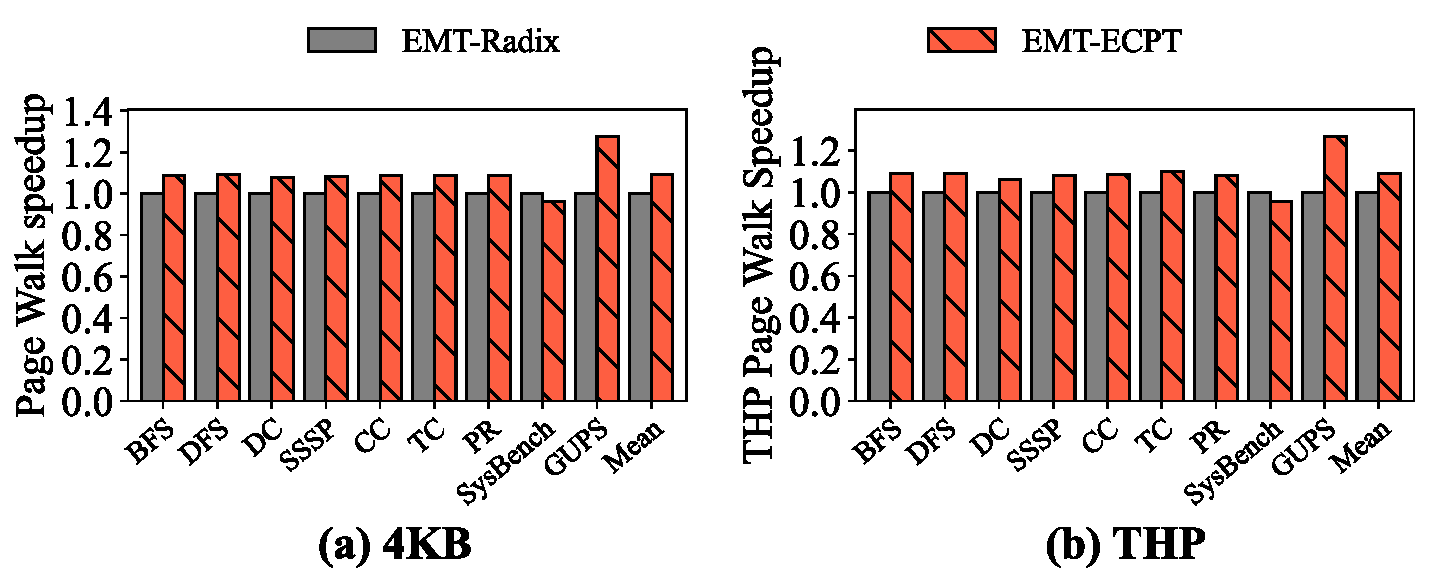
\includegraphics[width=0.49\textwidth]{data/ecpt}
% 	\caption{\bf Speedup of page walk in (a) 4KB and (b) THP of \eecpt over \eradix. \jyk{Replace EMT-Radix bars
% 	with a line. It saves space.}}
% 	%\vspace{-15pt}
% 	\label{emt:fig:eval:pw}
% \end{figure}

\end{comment}
% \begin{figure}
% 	\centering
% \begin{subfigure}[b]{0.45\textwidth}
% 	\centering
% 	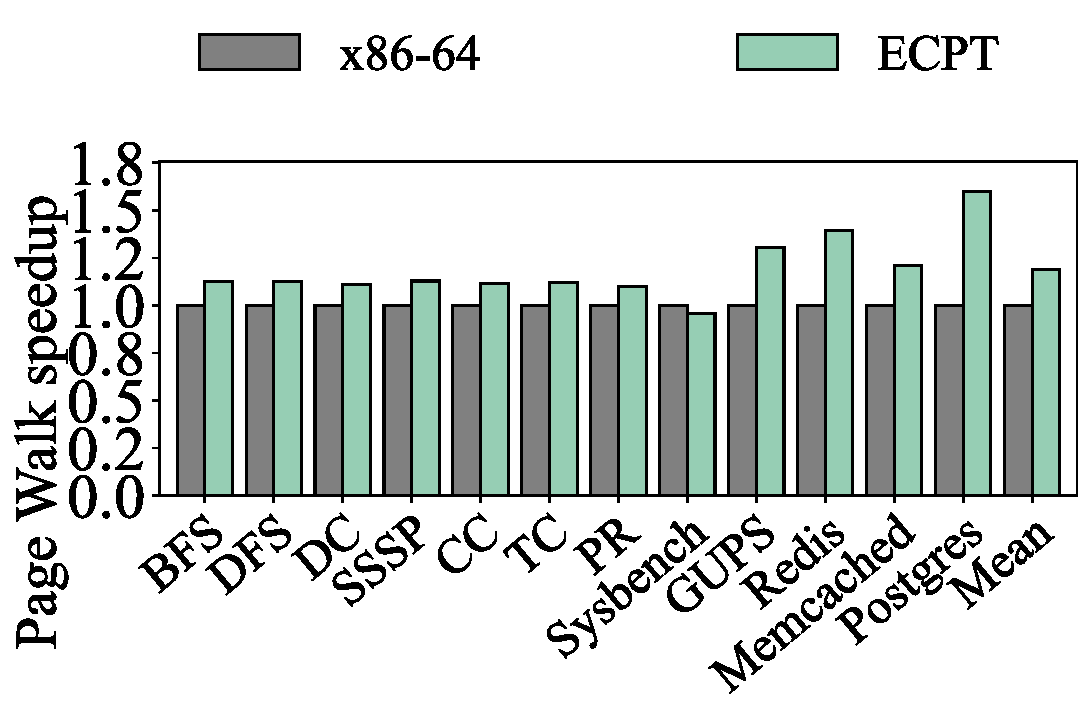
\includegraphics[width=\textwidth]{data/ecpt_pgwalk_never.pdf}
% 	% \vspace{-0.1cm}
% 	\vspace{-20pt}
% 	\caption{Page table walk latency}
% 	\label{emt:fig:eval:eval:pw-4KB}
% 	\end{subfigure}%
% 	% Subfigure 2
% 	% \vspace{-2cm}
% 	% \vspace{0.1cm}
% 	% \vspace{pt}
% 	\linebreak
% 	\begin{subfigure}[b]{0.45\textwidth}
% 	\centering
% 	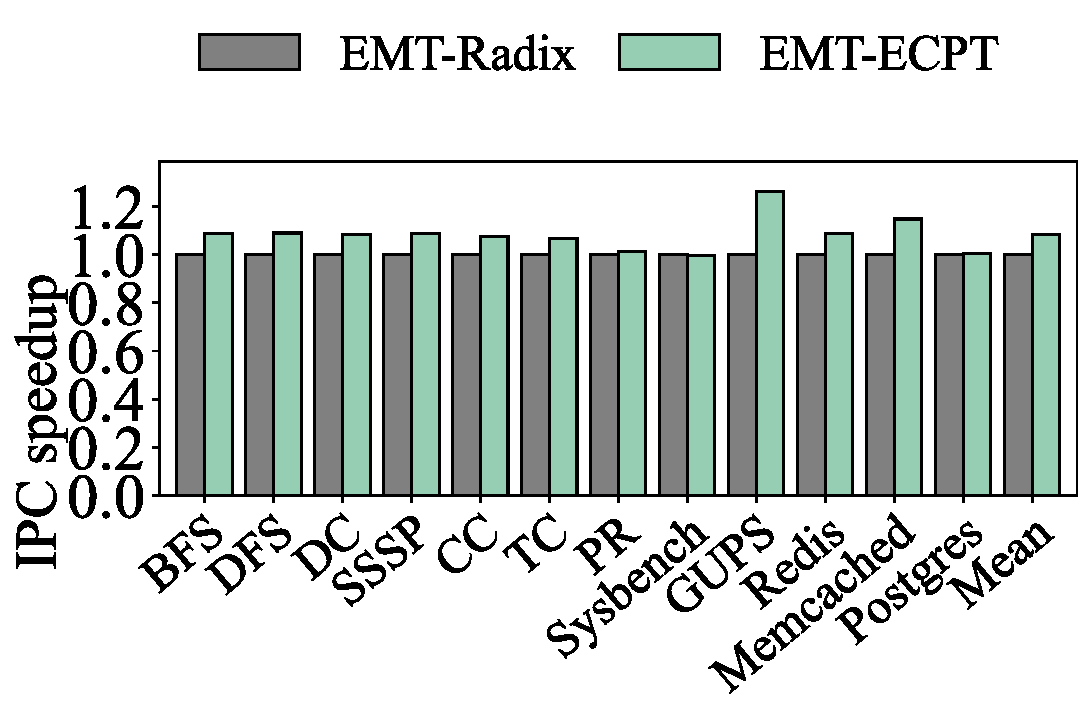
\includegraphics[width=\textwidth]{data/ecpt_ipc_never.pdf}
% 	% \vspace{-0.1cm}
% 	\vspace{-20pt}
% 	\caption{IPC}
% 	\label{emt:fig:eval:eval:ipc-4KB}
% 	\end{subfigure}

% 	\begin{subfigure}[b]{0.45\textwidth}
% 		\centering
% 		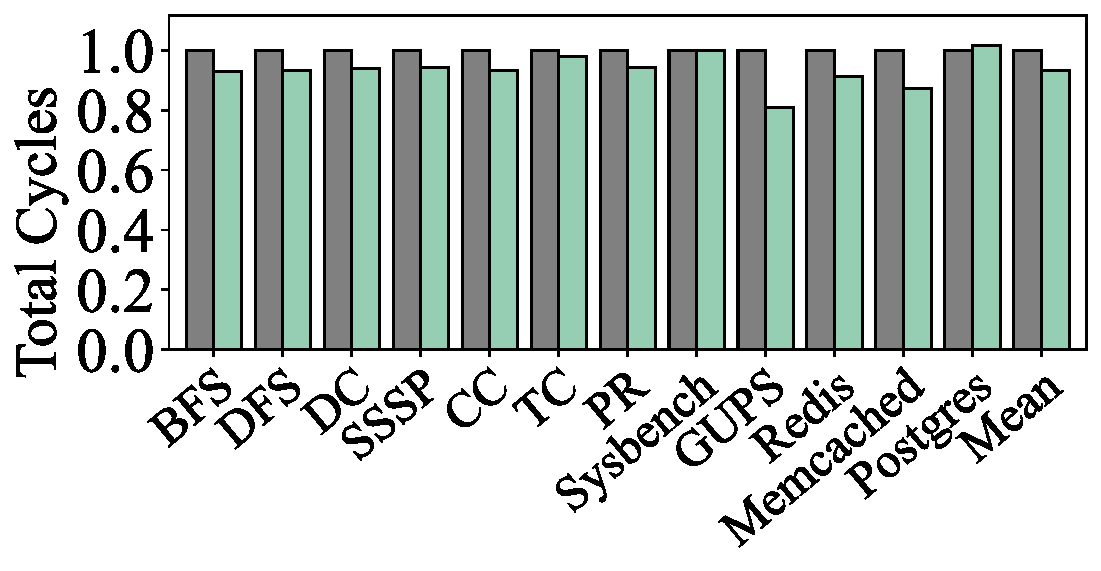
\includegraphics[width=\textwidth]{data/ecpt_e2e_never.pdf}
% 		% \vspace{-0.1cm}
% 		\vspace{-20pt}
% 		\caption{E2E}
% 		\label{emt:fig:eval:eval:e2e-4KB}
% 	\end{subfigure}

% 	\caption{\bf Speedup of page walk, IPC and E2E cycles for \eradix and \eecpt (running stage)}
% 	% \schaic{If we really need space, we can make EMT-radix as a line.}
% \end{figure}

\subsubsection{Hardware Simulation}
\label{emt:sec:eval:hwsim}

\paragraph{ECPT}

\noindent
EMT's emulator toolchain provides an open platform of hardware simulation
	for experimental architectures where silicon implementations are not available.
To demonstrate this, we run hardware simulations for EMT-Linux with the 
% \schaix{ECPT MMU and Radix drivers}
\schai{x86-64 radix and ECPT MMU drivers} using the DynamoRIO simulator~\cite{plat:dynamorio}.
	% using DynamoRIO~\cite{plat:dynamorio}. % (Figure~\ref{emt:fig:eval:emulator}).
We use the hardware configuration 
% \schaix{and simulation methodology} 
described in the ECPT paper~\cite{skarlatos2020ecpt}.
\schai{For PWC configuration, we follow more recent works~\cite{self:dmt,margaritov2019asap} to use 3 levels of PWC with 2-4-32 entries per level.}
We use the macro benchmarks and the three application workloads described in \S\ref{emt:sec:eval:metho}.
% \jz{
% We demonstrate that EMT can enable further insights when combined with existing hardware simulation infrastructures.
% EMT-Linux does not assume the execution platform,
%	so it can be run unmodified in the simulators commonly used in architectural research (e.g., gem5~\cite{plat:gem5}, DynamioRIO~\cite{plat:dynamorio}, SST~\cite{plat:sst}, or qemu~\cite{plat:qemu}).
% EMT can help researchers comprehensively evaluate their architectural designs including the software characteristics,
%	providing them with new understandings and insights,
%	without disrupting the hardware performance results.
% In this section, we demonstrate that the existing performance of ECPT can be reproduced
%	with full EMT-ECPT kernel implementation and the DynamioRIO hardware simulation framework~\cite{plat:dynamorio}.
% We then further demonstrate the software-related insights that we obtained based on the simulated result.}

% Unfortunately, ECPT doesn't yet have a silicon implementation, so we rely on simulator to evaluate its performance.
% Due to simluation constraint, we cannot sample the peformance of every instruction in the application. 
% Instead, we uniformly sampled over the life time of the application.
% \schaic{I provide how we do the unified approach for clarity. 
% 	For real submission, the division of loading and running stage may receive more attack than it should.
% 	I suggest we just mentioned we uniformly sampled the life time of the application in ultimate submission.}
% For each application's running and loading stage,
% 	we captured a trace containing 2B user instructions, kernel instructions happening during the 2B instructions,
% 	and all of their memory references.
% We fed each trace to DynamoRIO ~\cite{plat:dynamorio} to simulate page walk latency and data loading/writing latency
% 	similar to \cite{self:dmt,margaritov2019asap}, and then calculate total cycles and IPC based on the methodology outlined in next paragraph.
% We take a weighted average of loading and running stage cycles based on the number of user instructions in each stage
% 	(measured with perf on the real machine) to simulate a unified performance of the application.
% For example we caculate the total cycles by:
% 	% \[ total\_cycles = cycle\_load * (n\_inst\_load) + cycle\_run * (n\_inst\_runn) \]
% 	\begin{multline}
% 		total\_cycles =  \\
% 		\frac{cycle\_load * (n\_inst\_load) + cycle\_run * (n\_inst\_run)}{n\_inst\_load + n\_inst\_run}
% 	\end{multline}

% We reuse simulation configuration from original ECPT paper ~\cite{skarlatos2020ecpt} for DynamoRIO.
% Based on the simulation result, we calculate total cycles for each trace.
% For each instruction without data read/write, we treat its latency as half cycle execution time (~\cite{latency:instruction})
% 	plus its instruction fetching time which is iTLB time + page walk (if iTLB miss) + instruction fetching from memory.
% For each instruction with data read/write, we treat its latency dominated by its data read/write time
% 	which is TLB time + page walk (if TLB miss) + data read/write time.
% Adding up all the cycles for each instruction, we get the total cycles for each trace.
% We simulate a memory parallelism of 8 memory channels where data fetching happenning at the same time. 
% 	We divide the total data read/write time by the number of channles when calculating the total cycles.
% Then we divide the number of instructions over total cycles to get the IPC.
% % The simulator can calculate the  for each memory access
% % 	(~\cite{self:dmt})
% % We uniformly sampled over the life time of the application, captured trace with QEMU, 
% % 	and ran hardware simulation using DynamoRIO on the trace(Figure~\ref{emt:fig:eval:emulator}). 
% % We run hardware simulation using DynamoRIO with 
% % 	instruction and memory traces collected by our toolchain (Figure~\ref{emt:fig:eval:emulator}).


% % We measure page walk latency, instructions per cycles (IPC), and total cycles across the macro benchmarks 
% % 	and real world applications
% % 	running on the \eradix and \eecpt.
% % \schaic{We can remove the next sentence if we are worried that this may be poked. This is based on our improved methodology (confirmed with Dimitrios earlier) rather than the inaccurate one we used for last submission.}
% % Dynamo
% % Each non memory instruction is treated as half cycle (~\cite{latency:instruction})
% % 	and memory related instructions are treated as its page walk latency plus data loading/writing latency. 

% \jz{
% For the simulation, we use the DynamioRIO simulator~\cite{plat:dynamorio} 
%	seen in existing hardware research~\cite{self:dmt,margaritov2019asap,plat:dynamorio:copta},
%	as we cannot use the original ECPT simulation setup~\cite{skarlatos2020ecpt} due to its use of commercial simulator.
% We set the simulation parameters according to the original ECPT paper~\cite{skarlatos2020ecpt}.
% We reuse the applications we evaluated in previous sections (see \S\ref{emt:sec:eval:metho}) for consistency,
%	and they also largely overlap the ECPT-evaluated workloads~\cite{skarlatos2020ecpt}.
% For each application, we captured a trace containing 2 billion user instructions,
%	alongside all kernel instructions happening during the 2B instructions,
%	and all of their memory references.
% We fed each trace to DynamoRIO to simulate page walk latency and data loading/writing latency.
% Then, we calculate total cycles and IPC based on the methodology described in DMT~\cite{self:dmt},
%	the latest architecture work using the DynamioRIO simulator.
% }
\begin{figure}[tbp]
	\centering
	\begin{subfigure}[b]{0.6\textwidth}
		\centering
		
\includegraphics[width=\textwidth]{data/ecpt_legend.pdf}
	\end{subfigure}
	\vskip\baselineskip
	\begin{subfigure}[b]{0.48\textwidth}
		\centering
		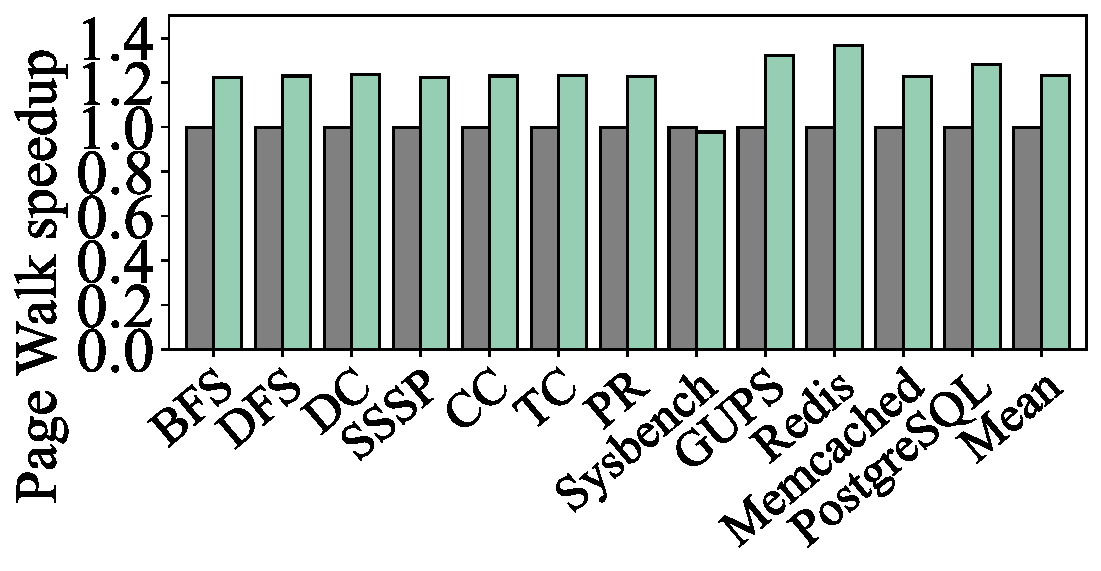
\includegraphics[width=\textwidth]{data/ecpt_pgwalk_unified_never.pdf}
		\caption{Page table walk latency}
		\label{emt:fig:eval:eval:pw-4KB}
	\end{subfigure}\hspace{0.02\textwidth}%
	\begin{subfigure}[b]{0.48\textwidth}
		\centering
		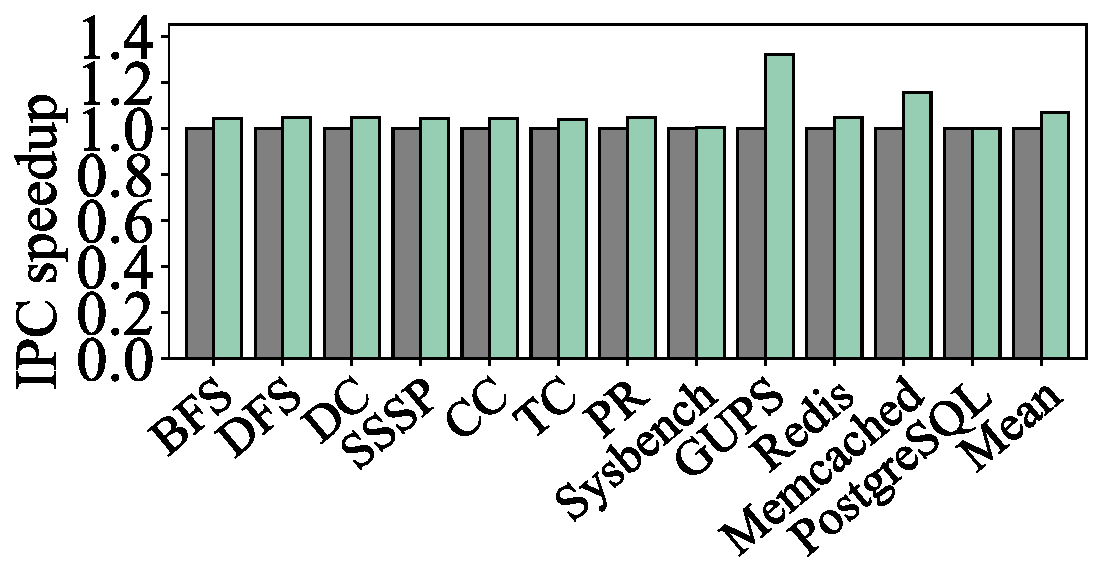
\includegraphics[width=\textwidth]{data/ecpt_ipc_unified_never.pdf}
		\caption{IPC}
		\label{emt:fig:eval:eval:ipc-4KB}
	\end{subfigure}
	\vskip\baselineskip
	\begin{subfigure}[b]{0.48\textwidth}
		\centering
		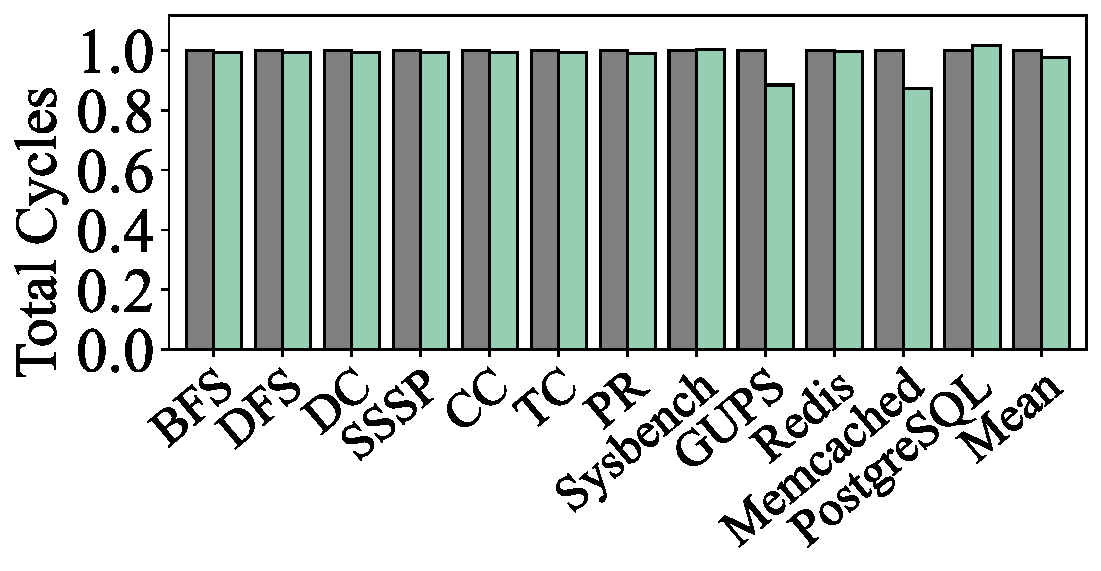
\includegraphics[width=\textwidth]{data/ecpt_e2e_unified_never.pdf}
		\caption{Total cycles}
		\label{emt:fig:eval:eval:e2e-4KB}
	\end{subfigure}\hspace{0.02\textwidth}%
	\begin{subfigure}[b]{0.48\textwidth}
		\centering
		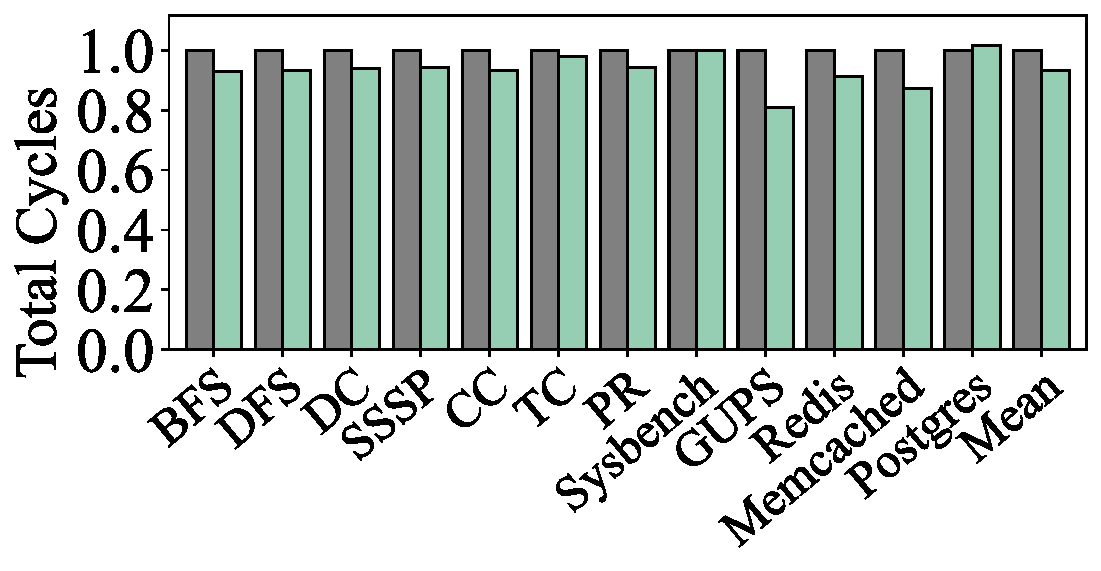
\includegraphics[width=\textwidth]{data/ecpt_e2e_never.pdf}
		\caption{Total cycles (running phase)}
		\label{emt:fig:eval:eval:e2ert-4KB}
	\end{subfigure}
\caption{{\bf ECPT hardware simulation results--- Page Table Walk Latency, 
    Instruction Per Cycle (IPC) and Total Cycles---with the ECPT system 
    and the x86-64 system, running EMT-Linux.} All results are normalized
    to those of the x86-64 system as the baselines.}
\label{emt:fig:hwsim}
% \vspace{-5pt}
\end{figure}

\schai{\para{Traditional Hardware Metrics.}}
Our toolchain measures traditional hardware metrics, namely 	
	Page Table Walk Latency and Instructions Per Cycle (IPC),
	which are considered 
	key performance metrics of hardware translation architectures (see~\cite{skarlatos2020ecpt,park2022fpt}).
% Figure~\ref{emt:fig:eval:eval:pw-4KB} and \ref{emt:fig:eval:eval:ipc-4KB}
%	shows the speedup of page walk latency and IPC of \eecpt over \eradix.
\schai{As shown in Figures~\ref{emt:fig:eval:eval:pw-4KB} and~\ref{emt:fig:eval:eval:ipc-4KB},
	ECPT has significant performance advantages over x86-64 (Radix).}
On average, ECPT speeds up page table walks by 23.1\%,
	and increases IPC by 7.0\%. %and end-to-end performance by 2.5 \%.
\schai{For most benchmarks, ECPT shows nontrivial page table walk and IPC speedups, 
	as it directly accesses the last-level PTEs.
%	without accessing intermediate page tables as radix does.
The only exception is Sysbench whose workload has a high PWC hit rate of 99.8\%
    at the PMD level on x86-64, i.e., 
	the x86-64 page table walks skip most intermediate steps and directly accesses last-level PTEs;
meanwhile, ECPT pays extra cycles for hash computation in addition to CWC accesses,
    so it slightly slows down Sysbench's page table walk by 2.2\%}

% The page walk speedup and IPC speedup are consistent with findings from the original ECPT paper~\cite{skarlatos2020ecpt},
% \jz{where the differences are attributed to difference in simulation platform~\cite{simaccuracy:sst,plat:simics}}.
% For most benchmarks, ECPT shows a page walk and IPC speedup because it directly fetches the final translation entry
% 	without accessing intermediate page tables as radix does.
% The only exception is Sysbench whose workload has a high PMD-PWC hit rate of 99.8\%, 
% 	so radix skips almost all of its steps and directly accesses its leaf level page table.
% Meanwhile, ECPT pays extra cycles for hash computation in addition to CWC accesses,
% so it has a slightly slower page table walk and IPC than radix.

\schai{\para{New Metrics with OS Overhead.}}
We find that IPC, which measures instruction throughput, does not fully 
	reflect application runtime---though
	ECPT increases IPC, our ECPT MMU driver introduces 
	more kernel instructions than the x86-64 MMU driver (\S\ref{emt:ss:eval:eval-ecpt-os}).
Hence, we measure the total cycles for running 
	macro benchmarks and applications,
	including the OS overhead (mostly page-fault handling as shown in Figure~\ref{emt:fig:eval:eval-kern-inst-breakdown}).
\schai{Figure~\ref{emt:fig:eval:eval:e2e-4KB} shows that},
	on average, the ECPT system reduces total cycles by 2.3\% across the workloads.
GUPS and Memcached show major benefits, where the ECPT system reduces the total cycles 
	by 11.5\% and 12.9\%, because 
\schai{page table walks account for over 66\% of their execution time.}
	% these two workloads involve 
	% \schaix{low kernel work.}
% \schai{significant proportion of page walk time.}
% \schaix{Detailed results are in Appendix~\ref{emt:sec:details_hwsim}}.

\schai{The aforementioned analysis shows that the OS can play 
    an important role in application performance,
    which could be overlooked with hardware metrics.
Without building the OS memory management, it is hard to evaluate 
	OS overhead accurately. 
Prior work assumed that OS overhead is constant under different memory-translation architectures. 
In the initial modeling, the memory trace is collected from running benchmarks 
	on vanilla Linux on x86-64; 
	the trace is then replayed in a simulator of ECPT MMU. 
As shown in \S\ref{emt:ss:perf-ecpt}, memory translation architectures can have profound implications for OS performance. 
% For example, in ECPT and other hashing-based translation schemes, range operations are inherently more expensive.
EMT aims to enable OS experience for new translation architectures.
We believe that EMT effectively lowers the barrier to implement OS support for new memory-translation architectures
by making the kernel developers focus on MMU driver implementations.}

\schai{
IPC as a metric aligns with application's execution time when OS overhead is minimal.
All the evaluated workloads have two phases:
a {\it loading phase} that loads data from the disk to memory,
and a {\it running phase} that runs the computation or serves user requests.
% We do not differentiate these fine-grained phases in our evaluation.
% The running phase often has lower kernel activities compared with the 
%     loading phase.
The running phase involves less kernel work with kernel instructions 
	accounting for less than 1.3\% of the total instructions.
% If we only consider the running phase, 
With only the running phase considered, ECPT 
    improves IPC by 7.5\% and reduces total cycles by 6.6\% 
	compared to the x86-64 system (Figure~\ref{emt:fig:eval:eval:e2ert-4KB}).
	
The results could be different with different hardware simulators.
We expect the impact of kernel instructions to become smaller 
	when using SST~\cite{plat:sst} which models OoO execution 
	more precisely. The SST evaluation remains future work.}


% \schaic{This modifications originated from reviewrC's comments on comparison with the original ECPT paper.}

% \jz{Based on the simulated result,
%	we further consider the impact of software overhead bring in by the ECPT kernel implemenation.
% We time the software overhead (\S\ref{emt:sec:eval:eval-EMT-radix-vs-vanilla} and \S\ref{emt:ss:perf-ecpt})
%	and the IPC (Figure~\ref{emt:fig:eval:eval:ipc-4KB}) to extrapolate the application runtime.}

% \jz{Figure~\ref{emt:fig:eval:eval:e2e-4KB} show the extrapolated end-to-end application runtime of \eecpt over \eradix.
% On average, ECPT speeds up application runtime by 2.5\%.
% We notice that} ECPT's IPC advantage is compromised by the high overhead in kernel memory management operations.
% As shown in Figure~\ref{emt:figure:eval:eval-kern-inst-breakdown-4k}, ECPT shows a 1.56x increase in kernel work
%	compared to radix.
% Its more complicated page table management routine leads to more kernel instructions while running the same user applications.
% The original ECPT doesn't reveal this signal since it focuses speedup analysis of user space instructions
%	\jz{and lack the tool to carry out the kernel performance analysis}.
% The original ECPT papger doesn't reveal this signal since it focuses on the stable stage of benchmarks which 
% 	contains less than 1\% of kernel instructions, so they are safe enough to ignore kernel impact.
% GUPS and Memcached are two outliers that show significant end-to-end performance speedup ()
%	since GUPS is dominated by page walk cycles and Memcached has lower kernel instruction ratio.
% The difference in IPC and end-to-end performance speedup reaffirms the importance of considering the kernel overhead
%	when designing a hardware MMU,
%	\jz{which motivates the developement and adoption of EMT
% }.
% On GUPS, Redis, and Memcached, ECPT shows 21\% to 39\% page walk speedup due to its large working set
% 	and scattered memory access patterns.
% With those applications, radix's leaf level page table access latency is similar to ECPT's;
% 	however, since radix's low PWC hit rate (e.g. 21\% for redis), radix pays extra steps to access intermediate page tables,
% 	which ECPT doesn't need to.
% Different from other benchmarks, ECPT doesn't show a page table walk speedup on sysbench.
% (2449917 + 344529) / 2800108 
% CSL: /disk/bak1/collect_trace_fast/radix/radix_never_sysbench_dyna_asplos_smalltlb_config_realpwc_2024-07-23_21-19-40.log

% ECPT increases application runtime IPC by 8.45\% on average
% 	(the original paper reported IPC increases of 11\%~\cite{skarlatos2020ecpt}).
% The gap comes from different simulator infrastructures.
%	we closely follow the implementation of ECPT and 
% The pattern of our macro benchmarks is that OS activities are heavy during 
% 	application bootstrapping (e.g., for loading data into memory)
% 	while user space dominates the application runtime (contributing to
% 	98.2\% of instructions).
% So ECPT's fast translation has significant performance benefits for most of the applications.

\begin{figure}[H]
	\centering
	\begin{subfigure}[b]{0.8\textwidth}
		\centering
		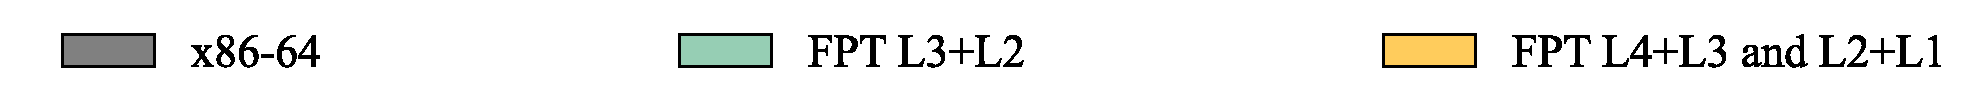
\includegraphics[width=\textwidth]{data/FPT_legend.pdf}
	\end{subfigure}
	\vskip\baselineskip
	\begin{subfigure}[b]{0.48\textwidth}
		\centering
		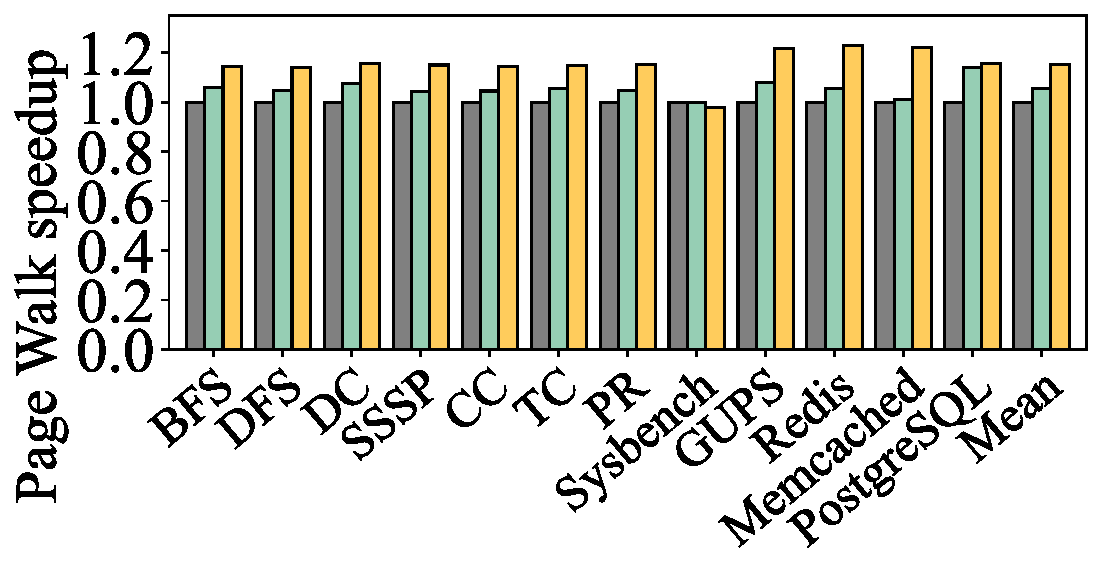
\includegraphics[width=\textwidth]{data/fpt_pgwalk_unified_never.pdf}
		\caption{Page table walk latency}
		\label{emt:fig:eval:eval:fpt-pw-4KB}
	\end{subfigure}\hspace{0.02\textwidth}%
	\begin{subfigure}[b]{0.48\textwidth}
		\centering
		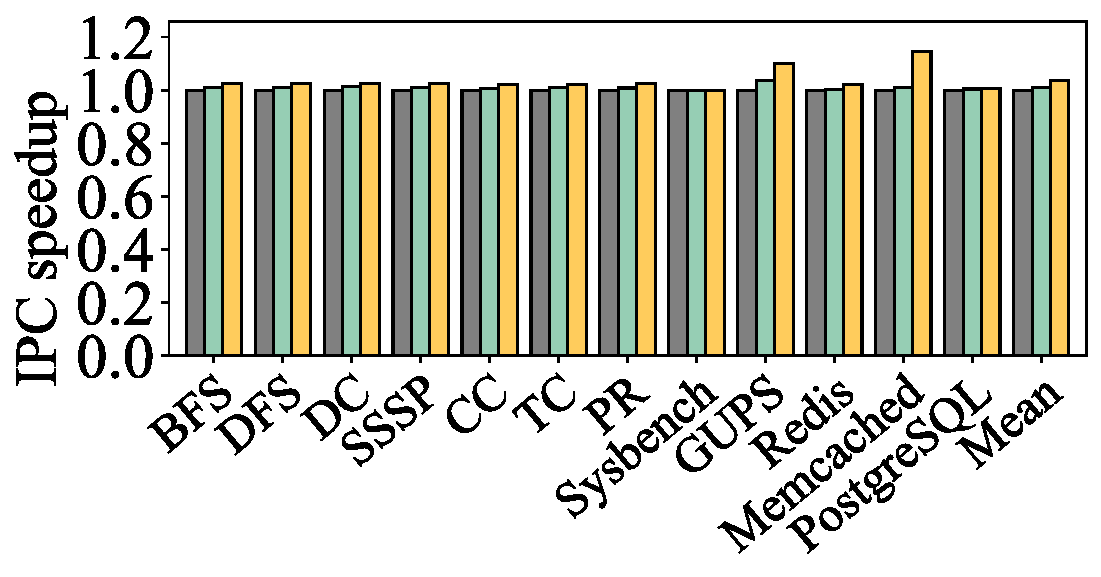
\includegraphics[width=\textwidth]{data/fpt_ipc_unified_never.pdf}
		\caption{IPC}
		\label{emt:fig:eval:eval:fpt-ipc-4KB}
	\end{subfigure}
	\vspace{-10pt}
	\vskip\baselineskip
	\begin{subfigure}[b]{0.48\textwidth}
		\centering
		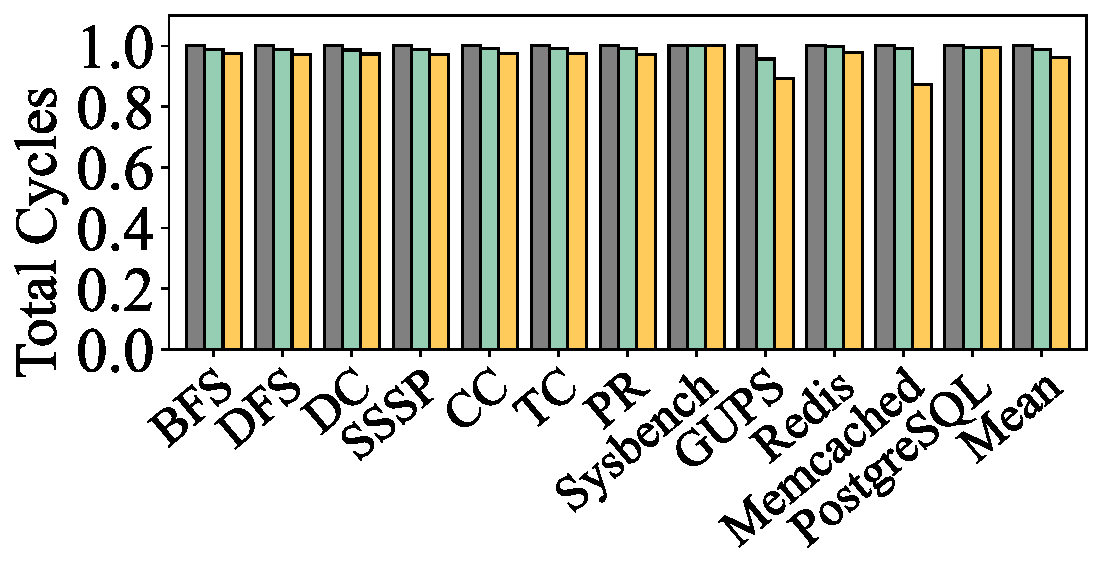
\includegraphics[width=\textwidth]{data/fpt_e2e_unified_never.pdf}
		\caption{Total cycles}
		\label{emt:fig:eval:eval:fpt-e2e-4KB}
	\end{subfigure}\hspace{0.02\textwidth}%
	\begin{subfigure}[b]{0.48\textwidth}
		\centering
		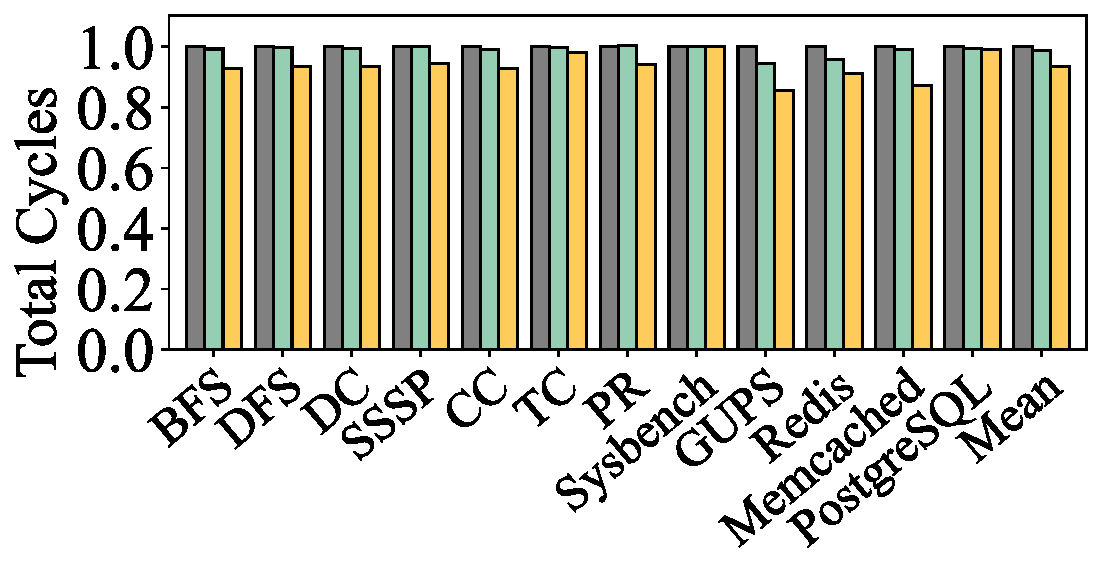
\includegraphics[width=\textwidth]{data/fpt_e2e_running_never.pdf}
		\caption{Total cycles (running phase)}
		\label{emt:fig:eval:eval:fpt-e2ert-4KB}
	\end{subfigure}
\caption{{\bf Hardware simulation results of the FPT system  
    and the x86-64 system, running EMT-Linux. } All results are normalized
    to those of the x86-64 system as the baselines.}
\label{emt:fig:hwsim-fpt}
% \vspace{-5pt}
\end{figure}

\paragraph{\schai{FPT}}
\label{emt:sec:eval:fpt}
% \noindent
% \para{FPT L3+L2.}
\noindent
\schai{We start with a FPT configuration 
	that flattens L3+L2 tables (see Figure~\ref{emt:fig:background:radix-native})
	which was implemented by the original OS prototype~\cite{park2022fpt}.
% We evaluated this configuration following the methodology in \S\ref{emt:sec:eval:hwsim}. 
Our evaluation shows that the benefit of flattening L3+L2 is limited: 
	only L3 entries were saved, which were cached effectively in x86-64. 
As shown in Figures~\ref{emt:fig:eval:eval:fpt-pw-4KB}, ~\ref{emt:fig:eval:eval:fpt-ipc-4KB},
	~\ref{emt:fig:eval:eval:fpt-e2e-4KB},
	compared with Linux on x86-64 (baseline), on average, 
	the FPT-based system speeds up page table walk latency by 5.5\%, IPC by 1.0\%, 
	and the total cycles by 1.1\%.}
% Only GUPS have non-trivial benefits, with the total cycles reduced by 4.3\% over the baseline.
% It also reduces OS overhead by 1.6\%.} % by reducing page table levels from 4 to 3.}

\schai{We then implemented the FPT configuration that flattens both L4+L3 and L2+L1.
This configuration was not implemented in~\cite{park2022fpt} 
	due to its difficulties of supporting 2MB huge pages.
We implemented a 4KB-only version and evaluated it with only 4KB base pages
	(no huge page).
%	was used in the hardware simulation in~\cite{park2022fpt}, %  of the original FPT paper
%	but not implemented due to the difficulty of supporting 2MB huge pages (Section 3.4 in~\cite{park2022fpt}).
With this configuration, compared with Linux on x86-64,
	the FPT-based system speeds up page table walk latency by 15.3\%, IPC by 3.6\%,
	and total cycles by 3.7\% (Figures~\ref{emt:fig:eval:eval:fpt-pw-4KB},~\ref{emt:fig:eval:eval:fpt-ipc-4KB}, and~\ref{emt:fig:eval:eval:fpt-e2e-4KB}).
% OS overhead by 3.4\%
% GUPS and Memcached benefit the most: their total cycles are reduced by 10.8\% and 12.7\% over the baseline.

% Interestingly, under this configuration, the FPT-based system leads to more total cycles reduction than the ECPT-based system, 
%	though the FPT-based system has lower page walk latency speedup and IPC speedup.
% The reason is that the FPT-based system has lower OS overhead
%	due to its simplified page table structure. 
% Compared with EMT-Linux on x86-64, under 4KB setup, the FPT-based system reduces OS overhead by 3.4\% on average,
% while the ECPT-based system increases OS overhead by 1.57x.

% We find that flattening L4+L3 and L2+L1 leads to similar performance with ECPT in the running phase.
Flattening both L4+L3 and L2+L1 in FPT yields performance comparable to ECPT in the running phase.
	% FPT reduces total cycles by 6.4\% and ECPT by 6.6\% (Figure ~\ref{emt:fig:eval:eval:fpt-e2ert-4KB} and~\ref{emt:fig:eval:eval:e2ert-4KB}).
Compared with radix, ECPT and FPT 
	reduce total cycles by 6.6\% and 6.4\%, respectively 
	(Figures~\ref{emt:fig:eval:eval:e2ert-4KB} and~\ref{emt:fig:eval:eval:fpt-e2ert-4KB}).
	% with matched hardware metrics.
	% However, FPT has a lower overall page table walk latency speedup and IPC speedup.
% This is caused by performance difference in different phases.
For hardware metrics (page table walk latency and IPC), 
	the FPT-based system matched ECPT-based system's performance:
ECPT is only faster than FPT by 2.4\% in page table walk latency and 0.4\% in IPC.
On the other hand, 
	ECPT inherently supports huge pages of varying sizes, unlike this FPT configuration.}

% Overall, under this configuration, the FPT- and ECPT-based systems achieve similar reductions of total cycles during the running phase
% 	FPT reduces total cycles by 6.4\% and ECPT by 6.6\%. 
% For the loading phase, the ECPT-based system is faster than the FPT-based system from an architecture perspective, with higher speedups on page-walk latency and IPC. 
% Meanwhile, the ECPT-based system has higher OS overhead; the OS overhead of the FPT-based system is slightly lower than the baseline (less than 1.5\% of kernel instructions on average).
